%% LyX 2.4.0~beta5 created this file.  For more info, see https://www.lyx.org/.
%% Do not edit unless you really know what you are doing.
\documentclass[english,footrule]{foils}
\usepackage[T1]{fontenc}
\usepackage[latin9]{inputenc}
\usepackage{geometry}
\geometry{verbose}
\setcounter{secnumdepth}{1}
\setcounter{tocdepth}{1}
\synctex=-1
\usepackage{xcolor}
\usepackage{babel}
\usepackage{url}
\usepackage{hepnames}
\usepackage{amsmath}
\usepackage{amsthm}
\usepackage{amssymb}
\usepackage{graphicx}
\usepackage[pdfusetitle,
 bookmarks=true,bookmarksnumbered=false,bookmarksopen=false,
 breaklinks=false,pdfborder={0 0 1},backref=false,colorlinks=false]
 {hyperref}

\makeatletter

%%%%%%%%%%%%%%%%%%%%%%%%%%%%%% LyX specific LaTeX commands.
\newcommand{\noun}[1]{\textsc{#1}}

%%%%%%%%%%%%%%%%%%%%%%%%%%%%%% Textclass specific LaTeX commands.
\theoremstyle{definition}
\newtheorem{defn}{\protect\definitionname}
\newenvironment{lyxcode}
	{\par\begin{list}{}{
		\setlength{\rightmargin}{\leftmargin}
		\setlength{\listparindent}{0pt}% needed for AMS classes
		\raggedright
		\setlength{\itemsep}{0pt}
		\setlength{\parsep}{0pt}
		\normalfont\ttfamily}%
	 \item[]}
	{\end{list}}

%%%%%%%%%%%%%%%%%%%%%%%%%%%%%% User specified LaTeX commands.
\usepackage{graphicx,xcolor}
% darker colors for better slides...
\definecolor{green}{RGB}{0, 180, 0}
\definecolor{cyan}{RGB}{0, 180, 180}
\definecolor{yellow}{RGB}{211,211,0}

%\usepackage{xcolor}
\renewcommand{\labelitemi}{$\textcolor{blue}{\bullet}$}
\renewcommand{\labelitemii}{$\textcolor{teal}{\Rightarrow}$}
\renewcommand{\labelitemiii}{$\textcolor{red}{\rightarrow}$}
\renewcommand{\labelitemiv}{$\textcolor{brown}{\circ}$}

\newcommand{\T}{\mathrm{T}}  % transpose
\newcommand{\PP}{\mathrm{P}}  % probability
\newcommand{\dd}{\mathrm{d}} % integration dx
\newcommand{\ee}{\mathrm{e}} % exponential
\newcommand{\E}{\mathrm{E}} % expectation


% DA
\newcommand{\xf}{\mathbf{x}^{\mathrm{f}}}
\newcommand{\xa}{\mathbf{x}^{\mathrm{a}}}
\newcommand{\xb}{\mathbf{x}^{\mathrm{b}}}
\newcommand{\xt}{\mathbf{x}^{\mathrm{t}}}
\newcommand{\barx}{\overline{\mathbf{x}}}

\newcommand{\M}{\mathbf{M}}
\newcommand{\Ho}{\mathbf{H}}

\newcommand{\x}{\mathbf{x}}
\newcommand{\y}{\mathbf{y}}
\newcommand{\yo}{\mathbf{y}^{\mathrm{o}}}
\newcommand{\bary}{\overline{\mathbf{y}}}

%\newcommand{\X}{\mathbf{X}}
\newcommand{\Xf}{\mathbf{X}_{\mathrm{f}}}
\newcommand{\Xa}{\mathbf{X}_{\mathrm{a}}}

%\newcommand{\bY}{\mathbf{Y}}
\newcommand{\Yf}{\mathbf{Y}_{\mathrm{f}}}

\newcommand{\w}{\mathbf{w}}
%\newcommand{\W}{\mathbf{W}}

\newcommand{\z}{\mathbf{z}}
\newcommand{\dv}{\mathbf{d}}

%\newcommand{\Pa}{\mathbf{P}^{\mathrm{a}}}
\newcommand{\Pf}{\mathbf{P}^{\mathrm{f}}}

\newcommand{\K}{\mathbf{K}}
%\newcommand{\B}{\mathbf{B}}
\newcommand{\R}{\mathbf{R}}
\newcommand{\Q}{\mathbf{Q}}
\newcommand{\X}{\mathbf{X}}
\newcommand{\bY}{\mathbf{Y}}
%\newcommand{\Ho}{\mathbf{H}}
\newcommand{\Hc}{\mathcal{H}}

%\newcommand{\M}{\mathbf{M}}
\newcommand{\Mc}{\mathcal{M}}
\newcommand{\Mk}{\mathbf{M}_{k}}
\newcommand{\Mkk}{\mathbf{M}_{k+1}}

\newcommand{\Rn}{\mathbb{R}^{n}}
\newcommand{\Rp}{\mathbb{R}^{p}}
\newcommand{\Rm}{\mathbb{R}^{m}}
\newcommand{\Rnn}{\mathbb{R}^{n\times n}}
\newcommand{\Rpp}{\mathbb{R}^{p\times p}}
\newcommand{\Id}{\mathbf{I}}

\newcommand{\ea}{\boldsymbol{\epsilon}^{\mathrm{a}}}
\newcommand{\eb}{\boldsymbol{\epsilon}^{\mathrm{b}}}
\newcommand{\ef}{\boldsymbol{\epsilon}^{\mathrm{f}}}
\newcommand{\eo}{\boldsymbol{\epsilon}^{\mathrm{o}}}
\newcommand{\eq}{\boldsymbol{\epsilon}^{\mathrm{q}}}

\newcommand{\zero}{\mathbf{0}}
\newcommand{\one}{\mathbf{1}}
\newcommand{\onehalf}{\frac{1}{2}}


\newcommand{\nn}{\nonumber\\}
\newcommand{\tr}{\rm Tr}
\def\({\left(}
\def\){\right)}

%\newcommand{\bu}{\mathbf{u}}
\newcommand{\baru}{\overline{\mathbf{u}}}
\newcommand{\bh}{\mathbf{h}}
\newcommand{\bv}{\mathbf{v}}
\newcommand{\bu}{\mathbf{u}}
\newcommand{\bz}{\mathbf{z}}

%\newcommand{\bP}{\mathbf{P}}
\newcommand{\bS}{\mathbf{S}}
%\newcommand{\bA}{\mathbf{A}}
\newcommand{\bV}{\mathbf{V}}
\newcommand{\bT}{\mathbf{T}}
%\newcommand{\bU}{\mathbf{U}}
\newcommand{\bE}{\mathbf{E}}
\newcommand{\bZ}{\mathbf{Z}}
\newcommand{\bC}{\mathbf{C}}
\newcommand{\bL}{\mathbf{L}}
\newcommand{\bP}{\mathbf{P}}


\newcommand{\bOmega}{\mathbf{\Omega}}
\newcommand{\bLambda}{\mathbf{\Lambda}}
\newcommand{\bdelta}{\bm{\delta}}
\newcommand{\brho}{\boldsymbol{\rho}}
\newcommand{\beps}{\boldsymbol{\epsilon}}
\newcommand{\bSigma}{\mathbf{\Sigma}}
\newcommand{\balpha}{\boldsymbol{\alpha}}
%\newcommand{\bbeta}{\bm{\beta}}
%\newcommand{\btheta}{\bm{\theta}}
\newcommand{\ceta}{\boldsymbol{\eta}}

%%MB
\newcommand{\Hess}{\mathrm{H}}
\newcommand{\Tc}{\mathcal{T}}

%%MA
%\newcommand{\dd}{\mathrm{d}}
\newcommand{\Pb}{\mathbf{P}^{\mathrm{b}}}

% operators
\newcommand{\argmin}{\operatornamewithlimits{argmin}} % for a "clean" argmin 
\newcommand{\argmax}{\operatornamewithlimits{argmax}} % for a "clean" argmax 
\DeclareMathOperator{\Tr}{Tr}  % for Trace of a matrix
\DeclareMathOperator{\Var}{Var}  % for the variance
\DeclareMathOperator{\Cov}{Cov}  % for the covariance
\DeclareMathOperator{\Cor}{Cor}  % for the covariance
\DeclareMathOperator{\Diag}{diag}  % for a diagonal matrix

\makeatother

\providecommand{\definitionname}{Definition}

\begin{document}
\title{Statistical Data Assimilation\\
\rule[0.5ex]{1\columnwidth}{3pt}}
\author{Mark Asch - CSU/IMU/2023}
\date{\bigskip{}
\bigskip{}
\bigskip{}
\noun{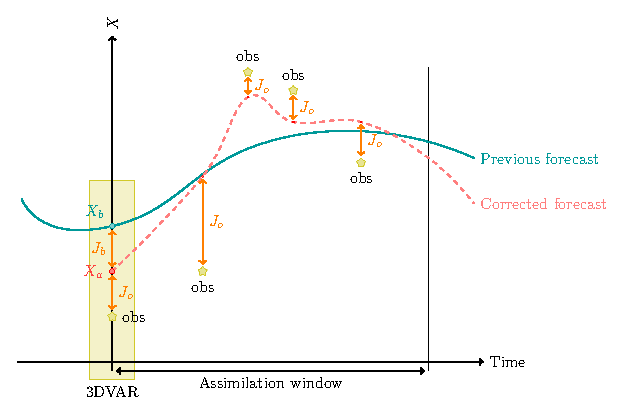
\includegraphics[scale=1.2]{graphics/3D4D-Var}}}
\maketitle

\MyLogo{Statistical Data Assim. - M. Asch - Lecture 04}

\foilhead{Outline of the course (I)}

\textcolor{blue}{Adjoint methods and variational data assimilation
(4h)}
\begin{enumerate}
\item Introduction to data assimilation: setting, history, overview, definitions.
\item \textcolor{lightgray}{Optimization methods.}
\item \textcolor{lightgray}{Adjoint method.}
\item \textcolor{lightgray}{Variational data assimilation methods: }
\begin{enumerate}
\item \textcolor{lightgray}{3D-Var, }
\item \textcolor{lightgray}{4D-Var.}
\end{enumerate}
\end{enumerate}

\foilhead{Outline of the course (II)}

\textcolor{blue}{Statistical estimation, Kalman filters and sequential
data assimilation (4h)}
\begin{enumerate}
\item \textcolor{red}{Introduction to statistical DA.}
\item \textcolor{red}{Statistical estimation.}
\item \textcolor{red}{The Kalman filter.}
\item Nonlinear extensions and ensemble filters.
\end{enumerate}

\foilhead{Reference Textbooks}
\begin{center}
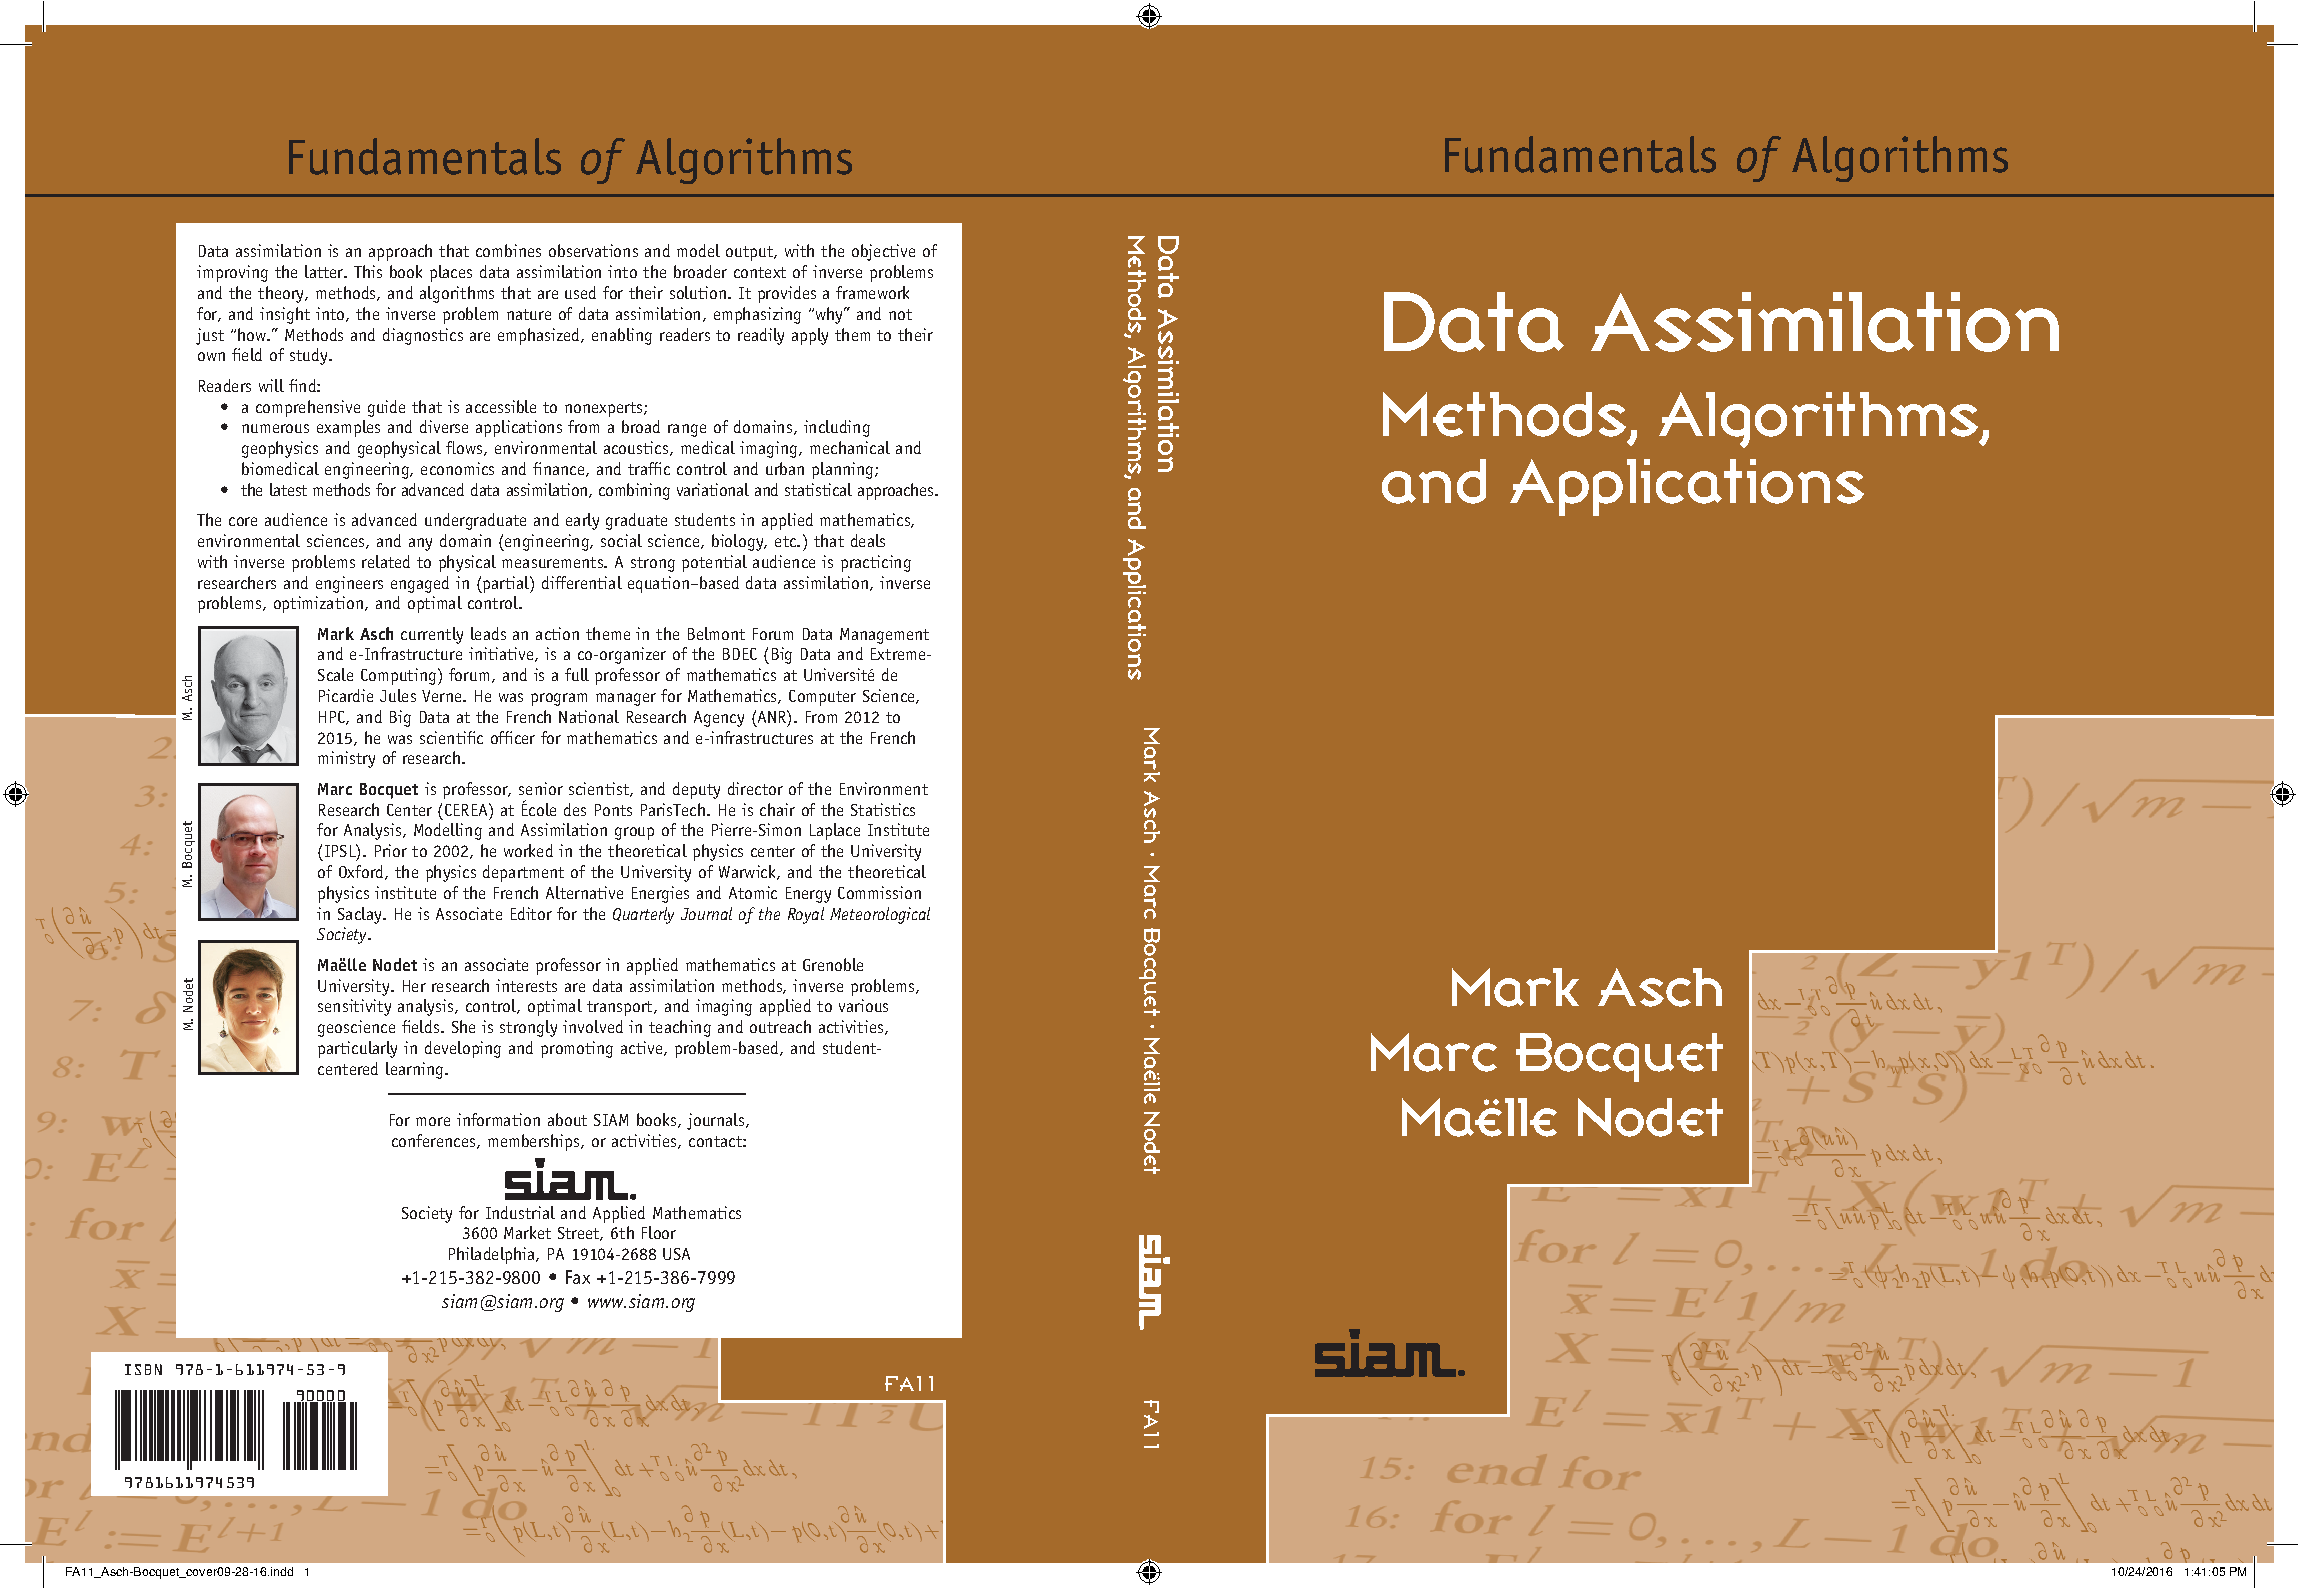
\includegraphics[width=0.8\textwidth]{graphics/FA11_Asch-Boucquet_cover10-24-16}
\par\end{center}

\begin{center}
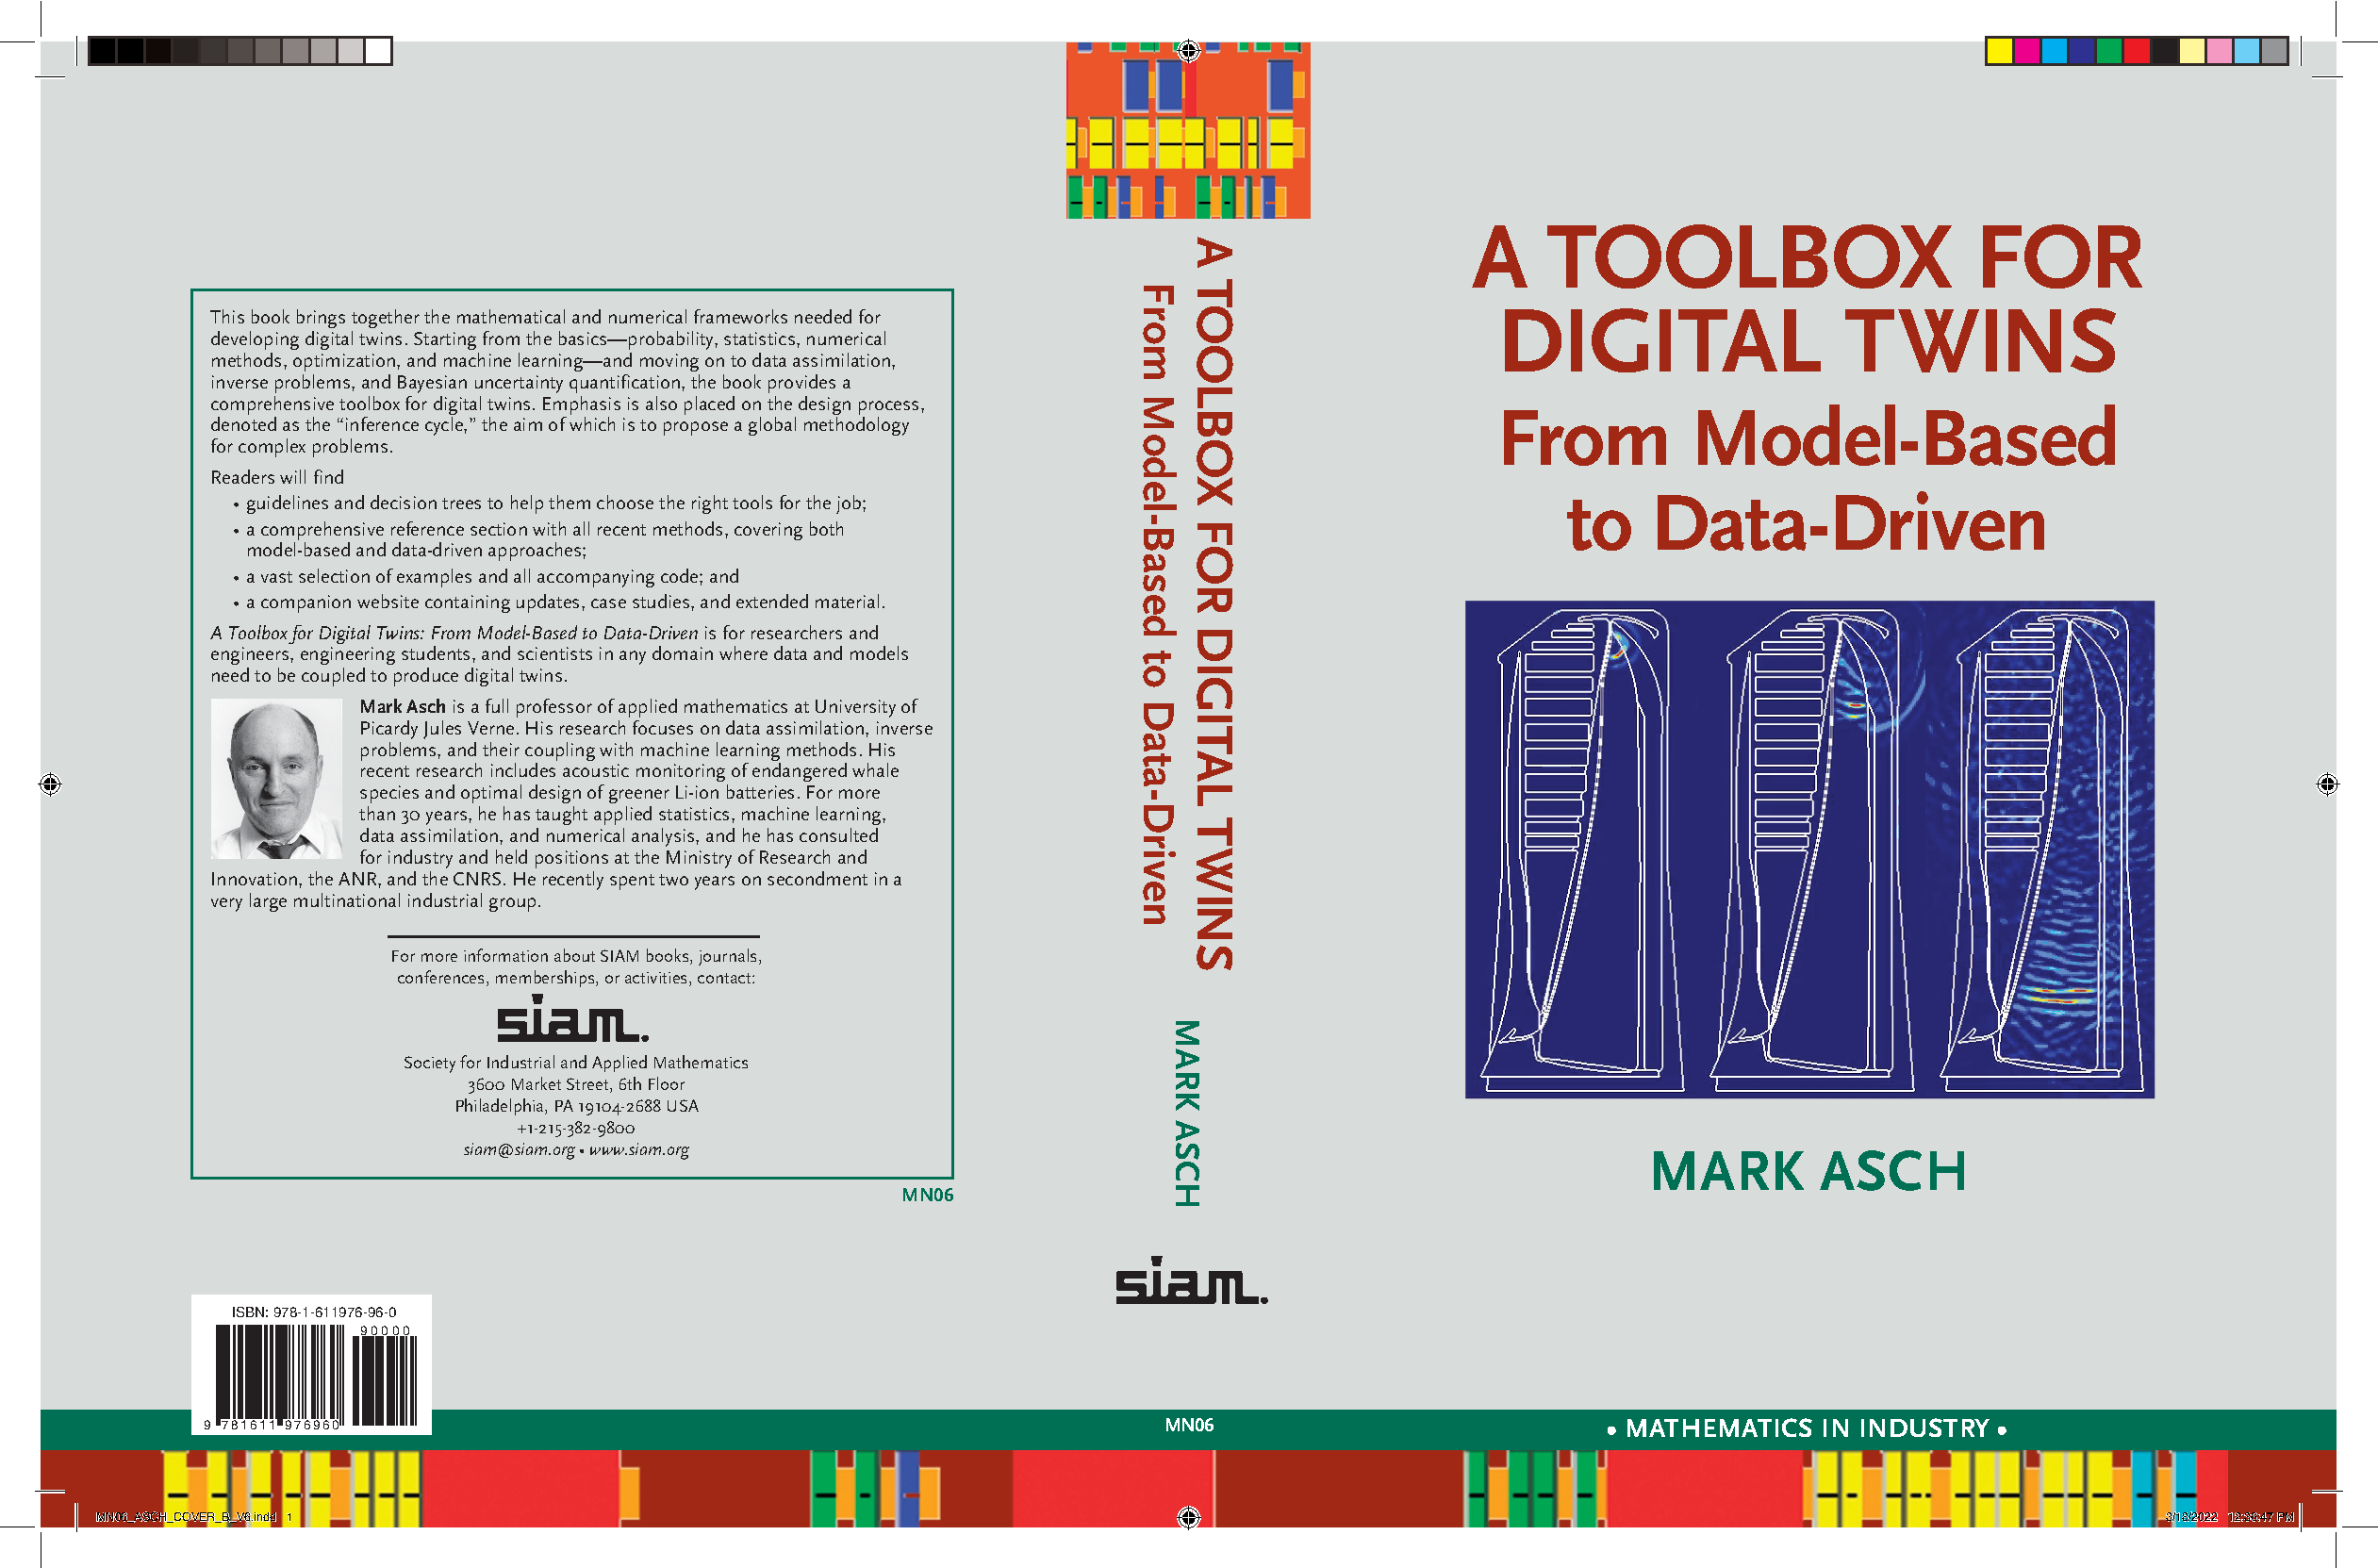
\includegraphics[width=0.8\textwidth]{graphics/MN06_ASCH_COVER_B_V6}
\par\end{center}

\foilhead{\textcolor{blue}{Statistical DA: introduction}}
\begin{itemize}
\item Now we will generalize the variational approach to deal with \textcolor{magenta}{errors
and noise} in 
\begin{itemize}
\item the models, 
\item the observations and 
\item the initial conditions. 
\end{itemize}
\item The variational results could of course be derived as a special case
of statistical DA, in the limit where the noise disappears.
\item Even the statistical results can be derived in a very general way,
using SDEs and/or Bayesian analysis, and then specialized to the various
Kalman-type filters that we will study here.
\item Practical inverse problems and data assimilation problems involve
measured data. 
\begin{itemize}
\item These data are inexact and are mixed with \textcolor{magenta}{random
noise}. 
\item Only \textcolor{magenta}{statistical models} can provide rigorous,
effective means for dealing with this measurement error.
\end{itemize}
\end{itemize}

\foilhead{\textcolor{blue}{Statistical DA: a ``simple'' example}}

We want to \textcolor{magenta}{estimate a scalar quantity}, say the
temperature or the ozone level, at a fixed point in space.

Suppose we have:
\begin{itemize}
\item a model forecast, $x^{\mathrm{b}}$ (\textcolor{blue}{background},
or \emph{a priori} value)
\item and a measured value, $x^{\mathrm{obs}}$ (\textcolor{blue}{observation}).
\end{itemize}
The simplest possible approach is to try a \textcolor{magenta}{linear
combination} of the two,
\[
x^{\mathrm{a}}=x^{\mathrm{b}}+w(x^{\mathrm{obs}}-x^{\mathrm{b}}),
\]
where $x^{\mathrm{a}}$ denotes the \textcolor{red}{analysis }that
we seek and $0\le w\le1$ is a \textcolor{magenta}{weight} factor.
We subtract the (always unknown) true state $x^{\mathrm{t}}$ from
both sides,
\[
x^{\mathrm{a}}-x^{\mathrm{t}}=x^{\mathrm{b}}-x^{\mathrm{t}}+w(x^{\mathrm{obs}}-x^{\mathrm{t}}-x^{\mathrm{b}}+x^{\mathrm{t}})
\]
and defining the three \textcolor{magenta}{errors} (analysis, background,
observation) as
\[
e^{\mathrm{a}}=x^{\mathrm{a}}-x^{\mathrm{t}},\quad\mathrm{e^{b}}=x^{\mathrm{b}}-x^{\mathrm{t}},\quad e^{\mathrm{obs}}=x^{\mathrm{obs}}-x^{\mathrm{t}},
\]
 we obtain
\[
e^{\mathrm{a}}=e^{\mathrm{b}}+w(e^{\mathrm{obs}}-e^{\mathrm{b}})=we^{\mathrm{obs}}+(1-w)e^{\mathrm{b}}.
\]
 If we have many realizations, we can take an \textcolor{magenta}{ensemble
average}, or expectation, denoted by $\left\langle \cdot\right\rangle ,$
\[
\left\langle e^{\mathrm{a}}\right\rangle =\left\langle e^{\mathrm{b}}\right\rangle +w(\left\langle e^{\mathrm{obs}}\right\rangle -\left\langle e^{\mathrm{b}}\right\rangle ).
\]
 Now if these errors are centred (have zero mean, or the estimates
of the true state are \textcolor{magenta}{unbiased}), then
\[
\left\langle e^{\mathrm{a}}\right\rangle =0
\]
also. So we must look at the \textcolor{magenta}{variance} and demand
that it be as small as possible. The variance is defined, using the
above notation, as 
\[
\sigma^{2}=\left\langle \left(e-\left\langle e\right\rangle \right)^{2}\right\rangle .
\]
Now, taking variances of the error equation, and using the zero-mean
property, we obtain
\[
\sigma_{\mathrm{a}}^{2}=\sigma_{\mathrm{b}}^{2}+w^{2}\left\langle \left(e^{\mathrm{obs}}-e^{\mathrm{b}}\right)^{2}\right\rangle +2w\left\langle e^{\mathrm{b}}\left(e^{\mathrm{obs}}-e^{\mathrm{b}}\right)\right\rangle .
\]
This reduces to 
\[
\sigma_{\mathrm{a}}^{2}=\sigma_{\mathrm{b}}^{2}+w^{2}\left(\sigma_{\mathrm{o}}^{2}+\sigma_{\mathrm{b}}^{2}\right)-2w\sigma_{\mathrm{b}}^{2}
\]
if $e^{\mathrm{o}}$ and $e^{\mathrm{b}}$ are \textcolor{magenta}{uncorrelated}. 

Now, to compute a \textcolor{magenta}{minimum}, take the derivative
with respect to $w$ and equate to zero, to obtain 
\[
0=2w\left(\sigma_{\mathrm{obs}}^{2}+\sigma_{\mathrm{b}}^{2}\right)-2\sigma_{\mathrm{b}}^{2},
\]
where we have ignored all cross terms (errors are assumed independent).
Finally, solving this last equation, we can write the \textcolor{red}{optimal
weight},
\[
w_{*}=\frac{\sigma_{\mathrm{b}}^{2}}{\sigma_{\mathrm{obs}}^{2}+\sigma_{\mathrm{b}}^{2}}=\frac{1}{1+\sigma_{\mathrm{o}}^{2}/\sigma_{\mathrm{b}}^{2}}
\]
 which depends on the \textcolor{magenta}{ratio} of the background
and the observation errors. Clearly $0\le w_{*}\le1$ and
\begin{itemize}
\item if the observation is perfect, $\sigma_{\mathrm{obs}}^{2}=0$ and
thus $w_{*}=1,$ the maximum weight;
\item if the background is perfect, $\sigma_{\mathrm{b}}^{2}=0$ and $w_{*}=0,$
so the observation will not be taken into account. 
\end{itemize}
We can now rewrite the analysis error variance as,
\begin{align*}
\sigma_{\mathrm{a}}^{2} & =w_{*}^{2}\sigma_{\mathrm{obs}}^{2}+(1-w_{*})^{2}\sigma_{\mathrm{b}}^{2}\\
 & =\frac{\sigma_{\mathrm{b}}^{2}\sigma_{\mathrm{obs}}^{2}}{\sigma_{\mathrm{obs}}^{2}+\sigma_{\mathrm{b}}^{2}}\\
 & =(1-w_{*})\sigma_{\mathrm{b}}^{2}\\
 & =\frac{1}{\sigma_{\mathrm{obs}}^{-2}+\sigma_{\mathrm{b}}^{-2}},
\end{align*}
where we suppose that $\sigma_{\mathrm{b}}^{2},\;\sigma_{\mathrm{o}}^{2}>0.$
In other words, 
\[
\frac{1}{\sigma_{\mathrm{a}}^{2}}=\frac{1}{\sigma_{\mathrm{o}}^{2}}+\frac{1}{\sigma_{\mathrm{b}}^{2}}.
\]
This is a very\textcolor{magenta}{{} fundamental result}, implying that
the overall \textcolor{magenta}{\emph{precision}}, $\tau=1/\sigma^{2},$
(reciprocal of the variance) is the sum of the background and measurement
precisions. Finally, the \textcolor{magenta}{analysis equation} becomes
\[
x^{\mathrm{a}}=x^{\mathrm{b}}+\frac{1}{1+\alpha}(x^{\mathrm{obs}}-x^{\mathrm{b}}),
\]
where $\alpha=\sigma_{\mathrm{obs}}^{2}/\sigma_{\mathrm{b}}^{2}.$
This is called the \textcolor{blue}{BLUE }- \textcolor{blue}{B}est
\textcolor{blue}{L}inear \textcolor{blue}{U}nbiased \textcolor{blue}{E}stimator
- because it gives an \textcolor{red}{unbiased, optimal weighting
for a linear combination} of two independent measurements.

\foilhead[-0.5in]{\textcolor{blue}{Statistical DA: 3 special cases and conclusions}}

We can isolate three special cases:
\begin{itemize}
\item if the observation is very accurate, $\sigma_{\mathrm{obs}}^{2}\ll\sigma_{\mathrm{b}}^{2},$
$\alpha\ll1$ and thus \textcolor{magenta}{$x^{\mathrm{a}}\approx x^{\mathrm{obs}}$}
\item if the background is accurate, $\alpha\gg1$ and\textcolor{magenta}{{}
$x^{\mathrm{a}}\approx x^{\mathrm{b}}$}
\item and finally, if observation and background varaiances are approximately
equal, $\alpha\approx1$ and $x^{\mathrm{a}}$ is the \textcolor{magenta}{arithmetic
average} of $x^{\mathrm{b}}$ and $x^{\mathrm{obs}}.$
\end{itemize}
\textbf{\textcolor{magenta}{Conclusion}}: this simple, linear model
does indeed capture the full range of possible solutions in a statistically
rigorous manner, thus providing us with an ``enriched'' solution when
compared with a non-probabilistic, scalar response such as the arithmetic
average of observation and background, which would correspond to only
the last of the above three special cases.

\foilhead{$\;$}

\vfill{}

\begin{center}
{\Large\textbf{\textcolor{blue}{KALMAN FILTERS}}}{\Large\par}
\par\end{center}

\vfill{}


\foilhead{Kalman Filters - background and history}
\begin{itemize}
\item DA is concerned with dynamic systems, where (noisy) observations are
acquired over time. 
\item \textcolor{magenta}{Question}: Is there some statistically optimal
way to combine the dynamic model and the observations? 
\item One \textcolor{magenta}{answer} is provided by \textcolor{magenta}{Kalman
filters} 
\begin{itemize}
\item They are linear models for state estimation of noisy dynamic systems. 
\item They have been the \emph{de facto} standard in many robotics and tracking/prediction
applications because they are well-suited for systems where there
is \textcolor{magenta}{uncertainty about an observable dynamic process}. 
\item They are also the basis of many data assimilation systems. 
\item They use a paradigm of \textcolor{red}{``observe, predict, correct''}
to extract information from a noisy signal.
\end{itemize}
\item The Kalman filter was invented\footnote{Apparently, following a prior invention by Stratonovich, one year
earlier.} in 1960 by R. E. K�lm�n to solve this sort of problem in a mathematically
optimal way. 
\item Its first use was on the Apollo missions to the moon, and since then
it has been used in an enormous \textcolor{magenta}{variety of domains}. 
\begin{itemize}
\item There are Kalman filters in aircraft and autonomous vehicles, on submarines,
and, in cruise missiles. 
\item Wall Street uses them to track the market. 
\item They are used in robots, in IoT (Internet of Things) sensors, and
in laboratory instruments. 
\item Chemical plants use them to control and monitor reactions. 
\item They are used to perform medical imaging and to remove noise from
cardiac signals. 
\item Weather forecasting is based on Kalman filters. 
\item They can effectively be used for modeling in \textcolor{magenta}{epidemiology}.
\end{itemize}
\item In \textcolor{magenta}{summary}, if it involves a sensor and/or time-series
data, a Kalman filter or a close relative of the Kalman filter is
usually involved.
\end{itemize}

\foilhead[-0.5in]{Kalman Filters - formulation}
\begin{itemize}
\item Consider a dynamical system that evolves in time and we would like
to\textcolor{magenta}{{} estimate }a series of \emph{true} states, $\xt_{k}$
(a sequence of random vectors) where discrete time is indexed by the
letter $k.$ 
\item These times are those when the \textcolor{magenta}{observations} or
measurements are taken, as shown in the Figure. 
\end{itemize}
\begin{figure}
\begin{centering}
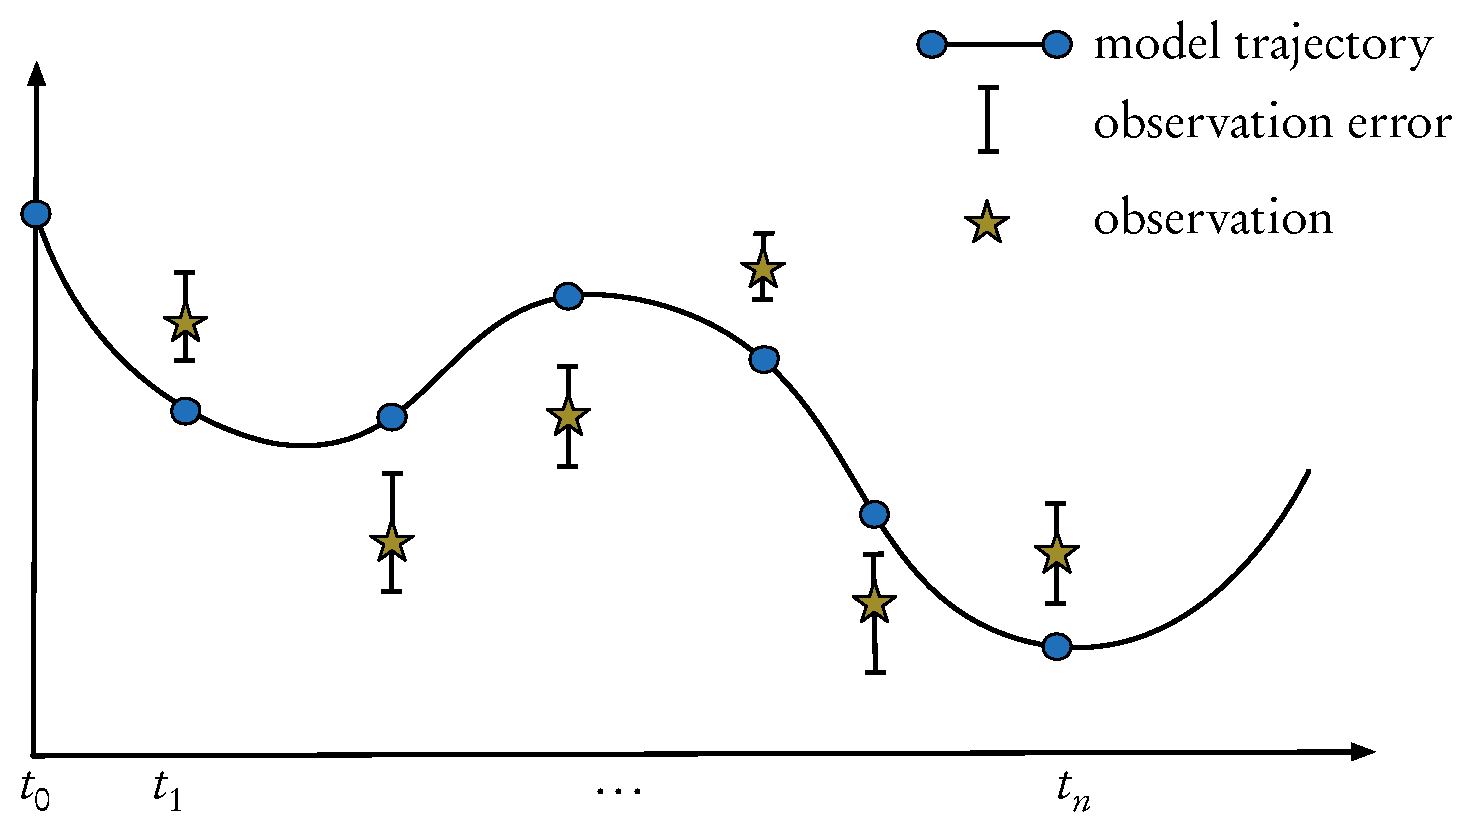
\includegraphics[width=0.8\textwidth]{graphics/mod_traject}
\par\end{centering}
\protect\caption[Sequential assimilation]{Sequential assimilation: a computed model trajectory, observations,
and their error bars.\protect\label{fig:Sequential-assimilation-1}}
\end{figure}

\begin{itemize}
\item The assimilation starts with an \textcolor{magenta}{unconstrained
model trajectory} from $t_{0},t_{1},\ldots,t_{k-1},t_{k},\ldots,t_{n}$
and aims to provide an\textcolor{magenta}{{} optimal fit }to the available
\textcolor{magenta}{observations/measurements} given their \textcolor{magenta}{uncertainties}
(error bars). 
\begin{itemize}
\item For example, in current, synoptic scale weather forecasts, $t_{k}-t_{k-1}=6$
hours and is less for the convective scale. 
\item In robotics, or autonomous vehicles, the time intervals are of the
order of the instrumental frequency, which can be a few milliseconds.
\end{itemize}
\end{itemize}

\foilhead{Kalman Filters - stochastic model}
\begin{itemize}
\item We seek to estimate the state $\x\in\mathbb{R}^{n}$ of a discrete-time
dynamic process that is governed by the\textcolor{magenta}{{} linear
stochastic difference equation} 
\begin{equation}
\x_{k+1}=\M_{k+1}\x_{k}+\mathbf{w}_{k}\label{eq:stateKF}
\end{equation}
\item with a \textcolor{magenta}{measurement/observation} $\y\in\mathbb{R}^{m},$
\begin{equation}
\mathbf{y}_{k}=\Ho_{k}\mathbf{x}_{k}+\mathbf{v}_{k}.\label{eq:obsKF}
\end{equation}
\item Note:
\begin{itemize}
\item $\M_{k+1}$ and $\Ho_{k}$ are considered linear, here. 
\item The random vectors, $\mathbf{w}_{k}$ and $\mathbf{v}_{k},$ represent
the process/modeling and measurement/observation errors respectively.
\item They are assumed to be independent, white noise processes with \textcolor{magenta}{Gaussian}/normal
probability distributions, 
\begin{eqnarray*}
\mathbf{w}_{k} & \sim & \mathcal{N}(0,\mathbf{Q}_{k}),\\
\mathbf{v}_{k} & \sim & \mathcal{N}(0,\mathbf{R}_{k}),
\end{eqnarray*}
where $\mathbf{Q}$ and $\mathbf{R}$ are the \textcolor{magenta}{covariance
matrices} (supposed known) of the modeling and observation errors
respectively. 
\end{itemize}
\item All these assumptions about unbiased and uncorrelated errors (in time
and between each other) are not limiting, since \textcolor{magenta}{extensions}
of the standard Kalman filter can be developed should any of these
not be valid\textemdash see Advanced Course.
\item We note that, for a broader mathematical view on the above system,
we could formulate all of statistical DA in terms of stochastic differential
equations (\textcolor{magenta}{SDEs}).\index{stochastic differential equations!data assimilation} 
\begin{itemize}
\item Then the theory of\textcolor{magenta}{{} It{�}} provides a detailed
solution of the problem of optimal filtering as well as rigorous existence
and uniqueness results... see {[}Law, Sarkka{]}.
\end{itemize}
\end{itemize}

\foilhead[-0.5in]{Kalman Filters - sequential assimilation scheme}

The typical assimilation scheme is made up of two major steps: 
\begin{enumerate}
\item a \textcolor{magenta}{prediction/forecast} step, and 
\item a \textcolor{magenta}{correction/analysis} step. 
\end{enumerate}
\begin{figure}
\index{Kalman filter!sequential assimilation|ffi}
\begin{centering}
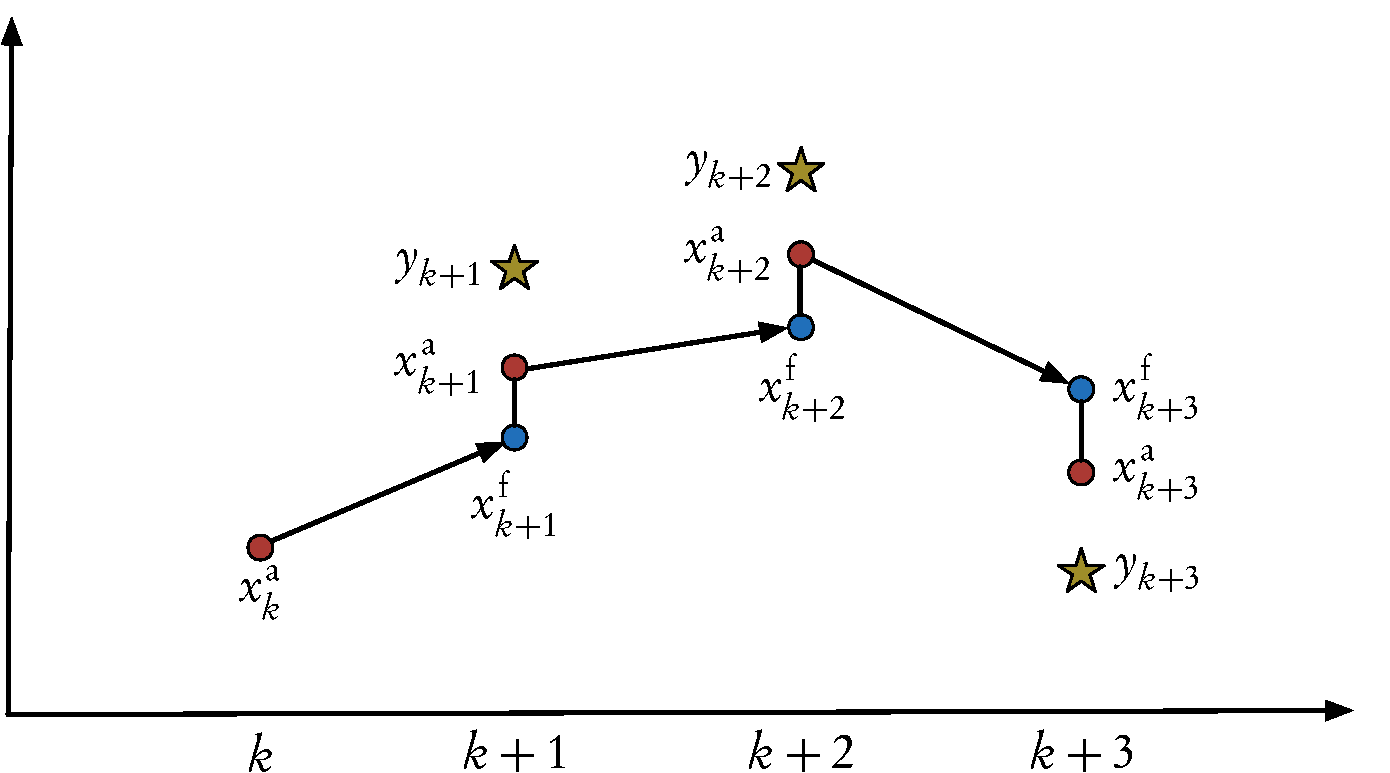
\includegraphics[width=0.8\textwidth]{graphics/seq_assim}
\par\end{centering}
\protect\caption[Sequential assimilation scheme for the Kalman filter]{Sequential assimilation scheme for the Kalman filter. The $x$-axis
denotes time, the $y$-axis denotes the values of the state and observations
vectors. \protect\label{fig:KFscheme-1}}
\end{figure}

\begin{itemize}
\item At time $t_{k}$ we have the result of a previous forecast, $\xf_{k},$
(the analogue of the background state $\xb_{k}$) and the result of
an ensemble of observations in $\y_{k}.$ 
\item Based on these two vectors, we perform an analysis that produces $\xa_{k}.$ 
\item We then use the evolution model to obtain a prediction of the state
at time $t_{k+1}.$ 
\item The result of the forecast is denoted $\xf_{k+1},$ and becomes the
background, or initial guess, for the next time-step\textemdash see
Figure \ref{fig:KFscheme-1}.
\item The Kalman filter problem can be resumed as follows: 
\begin{itemize}
\item given a prior/background estimate $\xf$ of the system state at time
$t_{k},$ 
\item what is the best update/analysis $\xa_{k}$ based on the currently
available measurements $\y_{k}?$
\end{itemize}
\end{itemize}

\foilhead[-0.5in]{Kalman Filters - the filter}
\begin{itemize}
\item The goal of the Kalman filter is:
\begin{itemize}
\item to compute \textcolor{magenta}{an optimal }\textcolor{magenta}{\emph{a
posteriori}}\textcolor{magenta}{{} estimate} $\mathbf{x}_{k}^{\mathrm{a}}$ 
\item that is a \textcolor{magenta}{linear combination} of an \emph{a priori}
estimate $\mathbf{x}_{k}^{\mathrm{f}}$ and a weighted difference
between the actual measurement $\mathbf{y}_{k}$ and the measurement
prediction $\mathbf{H}_{k}\xf_{k}.$ 
\end{itemize}
\item This is none other than the \textcolor{blue}{BLUE}\index{best linear unbiased estimator (BLUE)}
that we have seen above. 
\item The filter is thus of the linear, recursive form 
\begin{equation}
\mathbf{x}_{k}^{\mathrm{a}}=\mathbf{x}_{k}^{\mathrm{f}}+\mathbf{K}_{k}\left(\mathbf{y}_{k}-\mathbf{H}_{k}\mathbf{x}_{k}^{\mathrm{f}}\right).\label{eq:kfBlue-1}
\end{equation}

\begin{itemize}
\item The difference $\mathbf{d}_{k}=\mathbf{y}_{k}-\mathbf{H}_{k}\mathbf{x}_{k}^{\mathrm{f}}$
is called the\textcolor{magenta}{{} }\textcolor{magenta}{\emph{innovation}}\index{innovation}
and reflects the discrepancy between the actual and the predicted
measurements at time $t_{k}.$ 
\end{itemize}
\item Note that, for generality, the matrices are shown with a time-dependence.
When this is not the case, the subscripts $k$ can be dropped. The
\textcolor{magenta}{\emph{Kalman gain}}\textcolor{magenta}{{} matrix}\index{Kalman gain},
$\mathbf{K},$ is chosen to minimize the \emph{a posteriori} error
covariance equation (\ref{eq:apecov}).
\begin{itemize}
\item We define forecast (\emph{a priori}) and analysis (\emph{a posteriori})
estimate errors as 
\begin{eqnarray*}
\mathbf{e}_{k}^{\mathrm{f}} & = & \mathbf{x}_{k}^{\mathrm{f}}-\mathbf{x}_{k}^{\mathrm{t}},\\
\mathbf{e}_{k}^{\mathrm{a}} & = & \mathbf{x}_{k}^{\mathrm{a}}-\mathbf{x}_{k}^{\mathrm{t}},
\end{eqnarray*}
where $\mathbf{x}_{k}^{\mathrm{t}}$ is the (unknown) true state. 
\item Their respective error covariance matrices are 
\begin{eqnarray}
\mathbf{P}_{k}^{\mathrm{f}} & = & \Cov(\mathbf{e}_{k}^{\mathrm{f}})=\E\left[\mathbf{e}_{k}^{\mathrm{f}}(\mathbf{e}_{k}^{\mathrm{f}})^{\T}\right],\nonumber \\
\mathbf{P}_{k}^{\mathrm{a}} & = & \Cov(\mathbf{e}_{k}^{\mathrm{a}})=\E\left[\mathbf{e}_{k}^{\mathrm{a}}(\mathbf{e}_{k}^{\mathrm{a}})^{\T}\right].\label{eq:apecov}
\end{eqnarray}
\end{itemize}
\item To compute this \textcolor{magenta}{\emph{optimal gain}} requires
a careful derivation, that is beyond our scope here (see {[}Asch2016,
2022{]}).
\end{itemize}

\foilhead[-0.5in]{Kalman Filters - optimal gain}
\begin{itemize}
\item The \textcolor{magenta}{\emph{Kalman gain}}\textcolor{magenta}{{} matrix}\index{Kalman gain},
$\mathbf{K},$ is chosen to minimize the \emph{a posteriori} error
covariance equation (\ref{eq:apecov}).
\item The resulting $\mathbf{K}$ that minimizes equation (\ref{eq:apecov})
is given by 
\begin{equation}
\mathbf{K}_{k}=\mathbf{P}_{k}^{\mathrm{f}}\mathbf{H}_{k}^{\mathrm{T}}\left(\mathbf{H}_{k}\mathbf{P}_{k}^{\mathrm{f}}\mathbf{H}_{k}^{\mathrm{T}}+\mathbf{R}_{k}\right)^{-1},\label{eq:KFoptgain}
\end{equation}
where we remark that $\mathbf{H}\mathbf{P}_{k}^{\mathrm{f}}\mathbf{H}_{k}^{\T}+\mathbf{R}_{k}=\E\left[\mathbf{d}_{k}\mathbf{d}_{k}^{\T}\right]$
is the covariance of the innovation. 
\item Looking at this expression for $\mathbf{K}_{k},$ we see:
\begin{itemize}
\item when the measurement error covariance\textcolor{magenta}{{} $\mathbf{R}_{k}$
approaches zero}, the gain $\mathbf{K}_{k}$ weights the innovation
more heavily, since 
\[
\lim_{\mathbf{R}\rightarrow0}\mathbf{K}_{k}=\mathbf{H}_{k}^{-1}.
\]
\item On the other hand, as the \emph{a priori }error estimate covariance
\textcolor{magenta}{$\mathbf{P}_{k}^{\mathrm{f}}$ approaches zero},
the gain $\mathbf{K}_{k}$ weights the innovation less heavily, and
\[
\lim_{\mathbf{P}_{k}^{\mathrm{f}}\rightarrow0}\mathbf{K}_{k}=0.
\]
\item Another way of thinking about the weighting of $\mathbf{K}$ is that
as the measurement error covariance $\mathbf{R}$ approaches zero,
the actual measurement $\mathbf{y}_{k}$ is ``trusted'' more and
more, while the predicted measurement $\mathbf{H}_{k}\mathbf{x}_{k}^{\mathrm{f}}$
is trusted less and less. 
\item On the other hand, as the \emph{a priori} error estimate covariance
$\mathbf{P}_{k}^{\mathrm{f}}$ approaches zero, the actual measurement
$\mathbf{y}_{k}$ is trusted less and less, while the predicted measurement
$\mathbf{H}_{k}\mathbf{x}_{k}^{\mathrm{f}}$ is trusted more and more\textemdash this
will be illustrated in the computational example below.
\end{itemize}
\end{itemize}

\foilhead[-0.5in]{Kalman Filters - 2-step procedure}

\begin{figure}
\index{Kalman filter!implementation loop|ffi} 
\begin{centering}
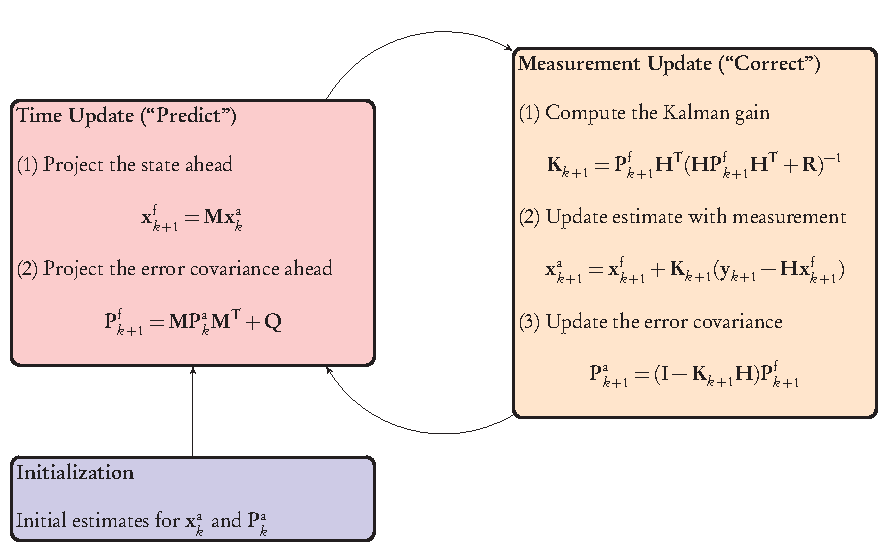
\includegraphics[width=1.1\textwidth]{graphics/KF-flow} 
\par\end{centering}
\protect\caption[Kalman filter loop]{Kalman filter loop, showing the two phases, predict and correct,
preceded by an initialization step.\protect\label{fig:kf_loop}}
\end{figure}

The predictor-corrector loop is illustrated in the Figure and can
be transposed, as is, into an\textcolor{magenta}{{} operational algorithm}.

\foilhead[-0.5in]{KF - \textcolor{blue}{predictor}/\textcolor{green}{forecast} step}
\begin{center}
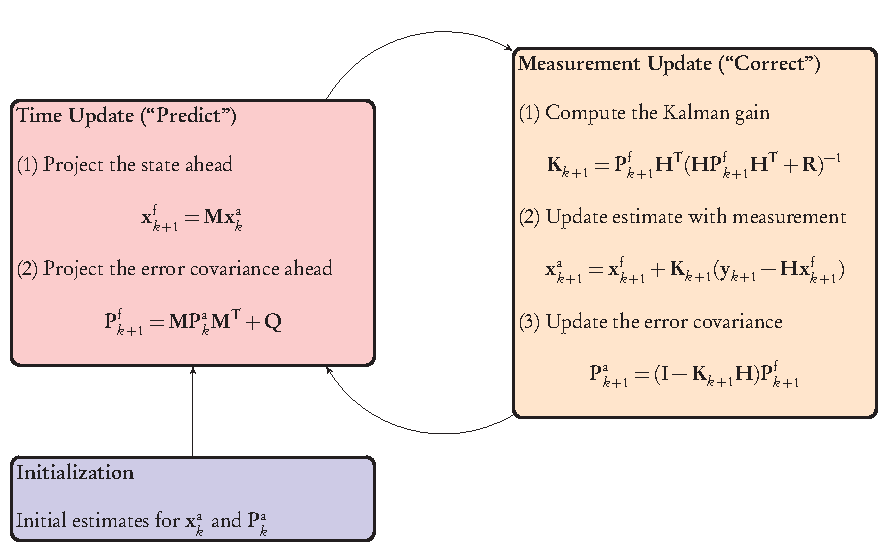
\includegraphics[width=0.5\textwidth]{graphics/KF-flow}
\par\end{center}
\begin{itemize}
\item Start from a previous analyzed state, $\mathbf{x}_{k}^{\mathrm{a}},$
or from the initial state if $k=0,$ characterized by the Gaussian
pdf $p(\mathbf{x}_{k}^{\mathrm{a}}\mid\mathbf{y}_{1:k}^{\mathrm{o}})$
of mean $\mathbf{x}_{k}^{\mathrm{a}}$ and covariance matrix $\mathbf{P}_{k}^{a}.$\footnote{We use here the classical notation $\mathbf{y}_{i:j}=(\mathbf{y}_{i},\mathbf{y}_{i+1},\ldots,\mathbf{y}_{j})$
for $i\le j$ that denotes conditioning on all the observations in
the interval. }
\item An estimate of $\mathbf{x}_{k+1}^{\mathrm{t}}$ is given by the dynamical
model which defines the forecast as 
\begin{eqnarray}
\mathbf{x}_{k+1}^{\mathrm{f}} & = & \mathbf{M}_{k+1}\mathbf{x}_{k}^{\mathrm{a}},\label{eq:fstate}\\
\mathbf{P}_{k+1}^{\mathrm{f}} & = & \mathbf{M}_{k+1}\mathbf{P}_{k}^{\mathrm{a}}\mathbf{M}_{k+1}^{\T}+\mathbf{Q}_{k+1},\label{eq:fcov1}
\end{eqnarray}
where the expression for $\Pf_{k+1}$ is obtained from the dynamics
equation and the definition of the model noise covariance, $\Q.$
\end{itemize}

\foilhead[-0.5in]{KF - \textcolor{blue}{corrector}/\textcolor{green}{analysis} step}
\begin{center}
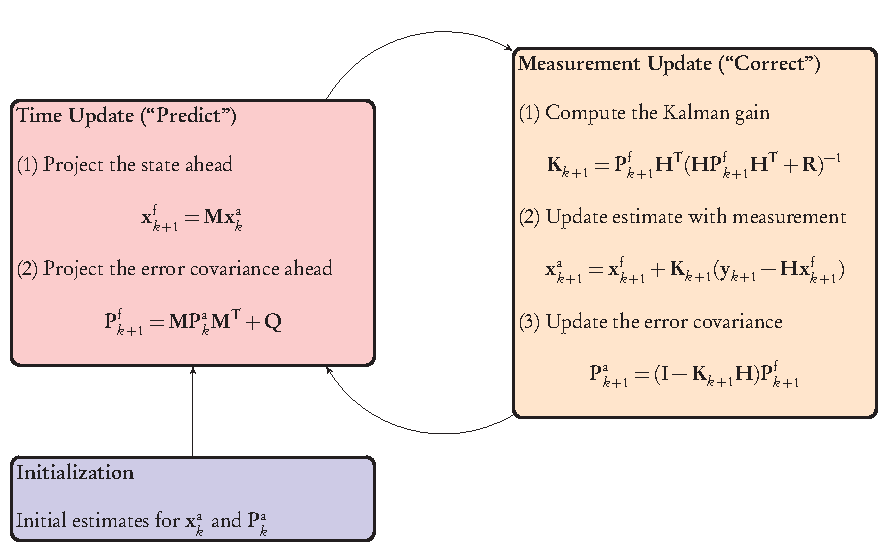
\includegraphics[width=0.5\textwidth]{graphics/KF-flow}
\par\end{center}
\begin{itemize}
\item At time $t_{k+1},$ the pdf $p(\mathbf{x}_{k+1}^{\mathrm{f}}\mid\mathbf{y}_{1:k}^{\mathrm{o}})$
is known, thanks to the mean $\mathbf{x}_{k+1}^{\mathrm{f}}$ and
covariance matrix $\mathbf{P}_{k+1}^{\mathrm{f}}$ just calculated,
as well as the assumption of a Gaussian distribution. 
\item The analysis step then consists of correcting this pdf using the observation
available at time $t_{k+1}$ in order to compute $p(\mathbf{x}_{k+1}^{\mathrm{a}}\mid\mathbf{y}_{1:k+1}^{\mathrm{o}}).$
This comes from the BLUE in the dynamical context and gives 
\begin{eqnarray}
\mathbf{K}_{k+1} & = & \mathbf{P}_{k+1}^{\mathrm{f}}\mathbf{H}^{\T}\left(\mathbf{H}\mathbf{P}_{k+1}^{\mathrm{f}}\mathbf{H}^{\T}+\mathbf{R}_{k+1}\right)^{-1},\label{eq:aK}\\
\mathbf{x}_{k+1}^{\mathrm{a}} & = & \mathbf{x}_{k+1}^{\mathrm{f}}+\mathbf{K}_{k+1}\left(\mathbf{y}_{k+1}-\mathbf{H}\mathbf{x}_{k+1}^{\mathrm{f}}\right),\label{eq:astate}\\
\mathbf{P}_{k+1}^{\mathrm{a}} & = & \left(\mathbf{I}-\mathbf{K}_{k+1}\mathbf{H}\right)\mathbf{P}_{k+1}^{\mathrm{f}}.\label{eq:acov}
\end{eqnarray}
\end{itemize}

\foilhead{KF - Overall Picture}
\begin{center}
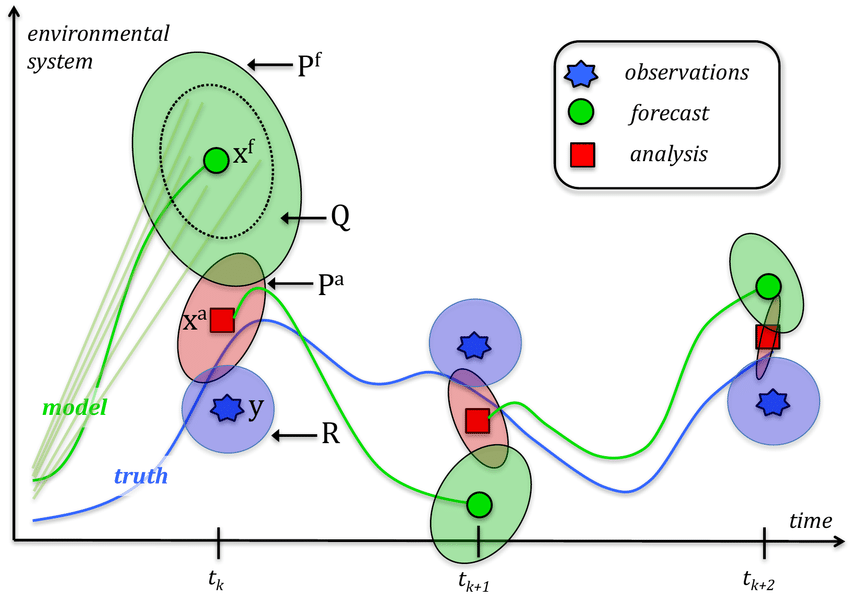
\includegraphics[width=1\textwidth]{graphics/Sketch-of-sequential-data-assimilation-algorithms-in-the-observation-space-where-H-is}
\par\end{center}

\textbf{Principle}: as we move forward in time, the uncertainty of
the analysis is reduced, and the forecast is improved.

\foilhead{KF - Relation Between Bayes and BLUE}
\begin{itemize}
\item If we know that the \emph{a priori} and the observation data are both
Gaussian, Bayes' rule can be readily applied to compute the \emph{a
posteriori} pdf. 
\begin{itemize}
\item The \emph{a posteriori} pdf is then Gaussian, and its parameters are
given by the BLUE equations. 
\end{itemize}
\item Hence with Gaussian pdfs and a linear observation operator, there
is no need to use Bayes' rule. 
\begin{itemize}
\item The BLUE equations can be used instead to compute the parameters of
the resulting pdf. 
\item Since the BLUE provides the same result as Bayes' rule, it is the
best estimator of all.
\end{itemize}
\item In addition one can recognize the 3D-Var cost function. 
\begin{itemize}
\item By optimizing this cost function, 3D-Var finds the MAP (maximum a
posteriori) estimate of the Gaussian pdf, which is equivalent to the
MV (minimum variance) estimate found by the BLUE.
\end{itemize}
\end{itemize}

\foilhead{$\;$}

\vfill{}

\begin{center}
{\Large\textbf{\textcolor{blue}{ENSEMBLE KALMAN FILTERS}}}{\Large\par}
\par\end{center}

\vfill{}


\foilhead{Ensemble Kalman Filter - EnKF}
\begin{itemize}
\item The ensemble Kalman filter (EnKF) is an elegant approach that avoids 
\begin{itemize}
\item the steps of \textcolor{magenta}{linearization} in the classical Kalman
Filter, 
\item and the need for \textcolor{magenta}{adjoints} in the variational
approach. 
\end{itemize}
\item It is still based on a Kalman filter, but an \textcolor{magenta}{ensemble
of realizations} is used to compute an estimate of the population
mean and variance, thus avoiding the need to compute inverses of potentially
large matrices to obtain the posterior covariance, as was the case
above in equations (\ref{eq:aK}) and (\ref{eq:acov}).
\item The EnKF and its variants have been successfully developed and implemented
in\textcolor{magenta}{{} meteorology and oceanography}, including in
operational weather forecasting systems. Because the method is simple
to implement, it has been widely used in these fields. 
\item But it has spread out to other geoscience disciplines and beyond.
For instance, to name a few domains, it has been applied in greenhouse
gas inverse modeling, air quality forecasting, extra-terrestrial atmosphere
forecasting , detection and attribution in climate sciences, geomagnetism
re-analysis , and ice-sheet parameter estimation and forecasting.
It has also been used in petroleum reservoir estimation, in adaptive
optics for extra large telescopes, and highway traffic estimation. 
\item More recently, the idea was proposed to exploit the EnKF as a universal
approach for all inverse problems. The term EKI, Ensemble Kalman Inversion,
is used to describe this approach. 
\end{itemize}

\foilhead{Principle of the EnKF}
\begin{itemize}
\item The EnKF was originally proposed by G. Evensen in 1994 and amended
in {[}Evenson2009{]}. 
\end{itemize}
\begin{defn}
The ensemble Kalman filter (EnKF) is a Kalman filter that uses an
ensemble of realizations to compute estimates of the population mean
and covariance.
\end{defn}
\begin{itemize}
\item Since it is based on \textcolor{magenta}{Gaussian} statistics (mean
and covariance) it does not solve the Bayesian filtering problem in
the limit of a large number of particles, as opposed to the more general
\emph{particle filter}\textemdash seeAdvanced Course. Nonetheless,
it turns out to be an excellent \textcolor{magenta}{approximate} algorithm
for the filtering problem.
\item As in the particle filter, the EnKF is based on the concept of particles,
a collection of state vectors, which are called the members of the
\textcolor{magenta}{ensemble}. 
\begin{itemize}
\item Rather than propagating huge covariance matrices, the errors are emulated
by scattered particles, a collection of state vectors whose variability
is meant to be representative of the uncertainty of the system's state
resulting from the forecaster's ignorance. 
\item Just like the particle filter, the members are propagated by the \textcolor{magenta}{nonlinear}
model, without any linearization. Not only does this avoid the derivation
of the tangent linear model, but it also circumvents the approximate
linearization. 
\item Finally, as opposed to the particle filter, the EnKF does not irremediably
suffer from the curse of dimensionality.\index{curse of dimensionality}
\end{itemize}
\item To sum up, here are the important remarks: 
\begin{itemize}
\item the EnKF avoids the \textcolor{magenta}{linearization} step of the
KF; 
\item the EnKF avoids the \textcolor{magenta}{inversion} of potentially
large matrices; 
\item the EnKF does not require any \textcolor{magenta}{adjoint}, as in
variational assimilation; 
\item the EnKF has been applied to a vast number of\textcolor{magenta}{{}
real-world }problems. 
\end{itemize}
\end{itemize}

\foilhead[-0.5in]{EnKF - the Three Steps}
\begin{enumerate}
\item \textbf{Initialization:} generate an ensemble of $m$ random states
$\left\{ \x_{i,0}^{\mathrm{f}}\right\} _{i=1,\ldots,m}$ at time $t=0.$ 
\item \textbf{Forecast:} compute the prediction for each member of the ensemble. 
\item \textbf{Analysis:} correct the prediction in light of the observations. 
\end{enumerate}
\begin{itemize}
\item Please see the Algorithm bleow for details of each step.
\item \textbf{Notes}:
\begin{enumerate}
\item Propagation can equivalently be performed either at the end of the
analysis step or at the beginning of the forecast step.
\item The Kalman gain is not computed directly, but \textcolor{magenta}{estimated}
from the ensemble statistics.
\item With the important exception of the Kalman gain computation, all operations
on the ensemble members are independent. As a result, \textcolor{magenta}{parallelization}
is straightforward. 
\item This is one of the main reasons for the \textcolor{magenta}{success/popularity}
of the EnKF. 
\end{enumerate}
\end{itemize}

\foilhead[-0.5in]{EnKF - Analysis Step}
\begin{itemize}
\item The EnKF seeks to mimic the analysis step of the Kalman filter but
with an \textcolor{magenta}{ensemble of limited size} in place of
the \textcolor{magenta}{unwieldy covariance matrices}. 
\item The goal is to perform for \textcolor{magenta}{each member} of the
ensemble an analysis of the form,
\begin{equation}
\x_{i}^{{\rm a}}=\x_{i}^{{\rm f}}+\K\left[\y_{i}-\Hc(\xf_{i})\right],\label{eq:member-update}
\end{equation}
where
\begin{itemize}
\item $i=1,\ldots,m$ is the member index in the ensemble,
\item $\xf_{i}$ is the forecast state vector $i$, which represents a background
state or prior at the analysis time.
\end{itemize}
\item To mimic the Kalman filter, $\K$ must be identified with the \textcolor{magenta}{Kalman
gain}
\begin{equation}
\K=\Pf\Ho^{\T}\ensuremath{\Ho\Pf\Ho^{\T}+\R}^{-1},\label{eq:kalman-gain}
\end{equation}
that we wish to \textcolor{magenta}{estimate from the ensemble statistics}. 
\begin{itemize}
\item First of all, we can estimate the\textcolor{magenta}{{} forecast error
covariance matrix }as a sum over the ensemble,
\[
\Pf=\frac{1}{m-1}\sum_{i=1}^{m}\left(\ensuremath{\x_{i}^{{\rm f}}-\barx^{{\rm f}}}\right)\left(\ensuremath{\x_{i}^{{\rm f}}-\barx^{{\rm f}}}\right)^{\T},
\]
with
\[
\barx=\frac{1}{m}\sum_{i=1}^{m}\x_{i}^{{\rm f}}.
\]
\item The forecast error covariance matrix can be \textcolor{magenta}{factorized}
into 
\[
\Pf=\Xf\Xf^{\T},
\]
where $\Xf$ is a $n\times m$ matrix whose columns are the \textcolor{magenta}{\emph{normalized
anomalies}} or \emph{normalized perturbations} \index{ensemble Kalman filter!perturbations}\index{ensemble Kalman filter!anomalies|see {perturbations}},
i.e. for $i=1,\ldots,m$ 
\[
\left[\Xf\right]_{i}=\frac{\x_{i}^{{\rm f}}-\barx^{{\rm f}}}{\sqrt{m-1}}.
\]
\end{itemize}
\item We can now obtain from (\ref{eq:member-update}) a \textcolor{magenta}{posterior
ensemble} $\left\{ \x_{i}^{{\rm a}}\right\} _{i=1,\ldots,m}$ from
which we can compute the posterior statistics. 
\item Hence, the \textcolor{magenta}{posterior state} and an ensemble of
\textcolor{magenta}{posterior perturbations} can be estimated from
\[
\barx^{{\rm a}}=\frac{1}{m}\sum_{i=1}^{m}\xa_{i}\,,\quad\left[\Xa\right]_{i}=\frac{\x_{i}^{{\rm a}}-\barx^{{\rm a}}}{\sqrt{m-1}}.
\]
\item Since $\y_{i}\equiv\y$ was assumed, the normalized anomalies, $\X_{i}^{{\rm a}}\equiv\left[\Xa\right]_{i}$,
i.e. the normalized deviations of the ensemble members from the mean
are obtained from (\ref{eq:member-update}) minus the mean update,
\begin{equation}
\X_{i}^{{\rm a}}=\X_{i}^{{\rm f}}+\K\left(\ensuremath{\zero-\Ho\X_{i}^{{\rm f}}}\right)=\left(\ensuremath{\Id_{n}-\K\Ho}\right)\X_{i}^{{\rm f}},\label{eq:anomaly-update}
\end{equation}

\begin{itemize}
\item where $\X_{i}^{{\rm f}}\equiv\left[\Xf\right]_{i}$, which yields
the \textcolor{magenta}{analysis error covariance matrix}, 
\begin{align*}
\bP^{{\rm a}} & =\Xa\Xa^{\T}\\
 & =(\Id_{n}-\K\Ho)\Xf\Xf^{\T}(\Id_{n}-\K\Ho)^{\T}\\
 & =(\Id_{n}-\K\Ho)\Pf(\Id_{n}-\K\Ho)^{\T}.
\end{align*}
\end{itemize}
\item Note that such a computation is never carried out in practice. However,
theoretically, in order to mimic the \textcolor{magenta}{best linear
unbiased estimator} (BLUE) analysis of the Kalman filter, we should
have obtained 
\begin{align*}
\bP^{{\rm a}} & =(\Id_{n}-\K\Ho)\Pf(\Id_{n}-\K\Ho)^{\T}+\K\R\K^{\T}\\
 & =(\Id_{n}-\K\Ho)\Pf.
\end{align*}

\begin{itemize}
\item Therefore, the error covariances are \textcolor{magenta}{underestimated}
since the second positive term, related to the observation errors,
is ignored, which is likely to lead to the \textcolor{magenta}{divergence}
of the EnKF when the scheme is cycled.
\end{itemize}
\item An elegant solution around this problem is to \textcolor{magenta}{perturb}
the observation vector for each member: $\y_{i}=\y+\bu_{i}$, where
$\bu_{i}$ is drawn from the Gaussian distribution $\bu_{i}\sim N(\zero,\R).$
\begin{itemize}
\item Let us define $\overline{\bu}$ the mean of the sampled $\bu_{i}$,
and the innovation perturbations
\begin{equation}
\left[\Yf\right]_{i}=\frac{\Ho\x_{i}^{{\rm f}}-\bu_{i}-\Ho\barx^{{\rm f}}+\baru}{\sqrt{m-1}}.\label{eq:innovation-pert}
\end{equation}
\item The \textcolor{magenta}{posterior anomalies} are modified accordingly,
\begin{equation}
\X_{i}^{{\rm a}}=\X_{i}^{{\rm f}}-\K\bY_{i}^{{\rm f}}=(\Id_{n}-\K\Ho)\X_{i}^{{\rm f}}+\frac{\K(\bu_{i}-\baru)}{\sqrt{m-1}}.\label{eq:anomaly-update-correction}
\end{equation}
\end{itemize}
\item These anomalies yield the \textcolor{magenta}{analysis error covariance
matrix}, 
\begin{align*}
\bP^{{\rm a}}= & (\Id_{n}-\K\Ho)\Pf(\Id_{n}-\K\Ho)^{\T}\\
 & +\K\left[\frac{1}{m-1}\sum_{i=1}^{m}(\bu_{i}-\baru)(\bu_{i}-\baru)^{\T}\right]\K^{\T}\\
 & +\frac{1}{\sqrt{m-1}}(\Id_{n}-\K\Ho)\Pf(\bu_{i}-\baru)^{\T}\K^{\T}\\
 & +\frac{1}{\sqrt{m-1}}\K(\bu_{i}-\baru)\Pf(\Id_{n}-\K\Ho)^{\T},
\end{align*}
whose expectation over the random noise gives the \textcolor{magenta}{proper}
expected \textcolor{magenta}{posterior covariances}, 
\begin{align*}
\E\left[\bP^{{\rm a}}\right] & =(\Id_{n}-\K\Ho)\Pf(\Id_{n}-\K\Ho)^{\T}\\
 & +\K\E\left[\frac{1}{m-1}\sum_{i=1}^{m}(\bu_{i}-\baru)(\bu_{i}-\baru)^{\T}\right]\K^{\T}\\
 & =(\Id_{n}-\K\Ho)\Pf(\Id_{n}-\K\Ho)^{\T}+\K\R\K\\
 & =(\Id_{n}-\K\Ho)\Pf.
\end{align*}
\item Note that the \textcolor{magenta}{gain} can be formulated in terms
of the anomaly matrices only, 
\begin{equation}
\K=\Xf\Yf^{\T}\left(\ensuremath{\Yf\Yf^{\T}}\right)^{-1},\label{eq:kalman-gain-pert}
\end{equation}
since 
\begin{itemize}
\item $\Xf\Yf^{\T}$ is a sample estimate for $\Pf\Ho^{\T}$ and 
\item $\Yf\bY_{{\rm f}}^{\T}$ is a sample estimate for $\Ho\Pf\Ho^{\T}+\R.$
\end{itemize}
\item In this form, it is striking that the updated perturbations are linear
combinations of the forecast perturbations. The new perturbations
are sought within the ensemble subspace of the initial perturbations. 
\item Similarly, the state analysis is sought within the affine space $\barx^{{\rm f}}+\mathrm{Vec}\left(\ensuremath{\X_{1}^{{\rm f}},\X_{2}^{{\rm f}},\ldots,\X_{m}^{{\rm f}}}\right).$
\end{itemize}

\foilhead[-0.5in]{EnKF - Forecast Step}
\begin{itemize}
\item In the forecast step, the updated ensemble obtained at the analysis
step is \textcolor{magenta}{propagated} by the model over a time step,
\[
\mbox{for}\quad i=1,\ldots,m\quad\x_{i,k+1}^{{\rm f}}=\Mc_{k+1}(\xa_{i,k}).
\]
\item A forecast can be computed from the mean of the\textcolor{magenta}{{}
forecast ensemble}, while the forecast error covariances can be estimated
from the forecast perturbations. 
\item Notyes:
\begin{itemize}
\item These are only optional diagnostics in the scheme and they are not
required in the cycling of the EnKF. 
\item It is important to observe that using the \textcolor{magenta}{tangent
linear model }(TLM) operator, or any linearization thereof, was \textcolor{red}{avoided}. 
\item This difference should particularly matter in a significantly \textcolor{magenta}{nonlinear}
regime. 
\item However, as we shall see in the Advanced Course Lectures, in strongly
nonlinear regimes, the EnKF is largely dominated by schemes known
as the iterative EnKF\index{iterative ensemble Kalman filter} and
the iterative ensemble Kalman smoother
\end{itemize}
\end{itemize}

\foilhead{Comparison: EnKf and 4D-Var}
\begin{center}
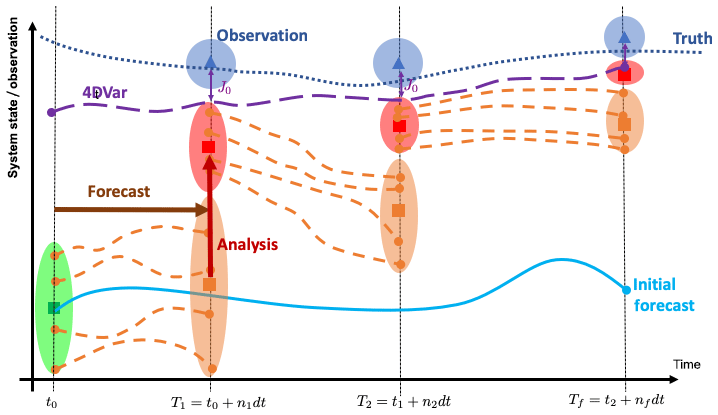
\includegraphics[width=0.8\textwidth]{graphics/enKF_4DVar}
\par\end{center}
\begin{itemize}
\item \textcolor{magenta}{Principle} of data assimilation: Having a physical
model able to forecast the evolution of a system from time $t=t_{0}$
to time$t=T_{f}$ (cyan curve), the aim of DA is to use available
observations (blue triangles) to correct the model projections and
get closer to the (unknown) truth (dotted line). 
\item In \textcolor{magenta}{EnKF}s, the initial system state and its uncertainty
(green square and ellipsoid) are represented by $m$ members. 
\begin{itemize}
\item The \textcolor{magenta}{members are propagated} forward in time during
$n_{1}$ model time steps $dt$ to $t=T_{1}$ where observations are
available (forecast phase, orange dashed lines). 
\item At $t=T_{1}$ the analysis uses the observations and their uncertainty
(blue triangle and ellipsoid) to produce a new system state that is
\textcolor{magenta}{closer to the observations} and with a \textcolor{magenta}{lower
uncertainty} (red square and ellipsoid). 
\item A \textcolor{magenta}{new forecast }is issued from the analyszd state
and this procedure is repeated until the end of the assimilation window
at $t=T_{f}.$ 
\item The model state should get closer to the truth and with lower uncertainty
as more observations are assimilated. 
\end{itemize}
\item Time-dependent variational methods (\textcolor{magenta}{4D-Var}) iterate
over the assimilation window to find the trajectory that minimises
the misfit ($J_{0}$) between the model and all observations available
from $t_{0}$ to $T_{f}$ (violet curve). 
\item For \textcolor{magenta}{linear dynamics, Gaussian errors and infinite
ensemble sizes}, the states produced at the end of the assimilation
window by the two methods should be equivalent (Li and Navon, 2001).
\end{itemize}

\foilhead{EnKF - the Algorithm}
\begin{lyxcode}
{\scriptsize\textbf{Given}}{\scriptsize :~For~$k=0,\ldots,K,$~observation~error~cov.~matrices}{\scriptsize\par}

{\scriptsize ~~~~~~~~~~~~$\R_{k}$,~observation~models~$\Hc_{k}$,~forward~models~$\Mc_{k}.$~}~\\
{\scriptsize\textbf{Compute}}{\scriptsize :~the~ensemble~forecast~$\left\{ \x_{i,k}^{\mathrm{f}}\right\} _{i=1,\ldots,m,\,k=1,\ldots,K}$~}{\scriptsize\par}

{\scriptsize$\left(\x_{i,0}^{\mathrm{f}}\right)_{i=1,\ldots,m}$~~~~~~~~~~~~\#Initialize~the~ensemble}{\scriptsize\par}

{\scriptsize for~$k=0$~to~$K$~do~~~~~~~~\#Loop~over~time}{\scriptsize\par}

{\scriptsize ~~for~~$i=1$~to~$m$~do~\#Draw~a~stat.~consistent~obs.~set}{\scriptsize\par}

{\scriptsize ~~~~$\bu_{i}\sim{\cal N}(0,\R_{k})$}{\scriptsize\par}

{\scriptsize ~~~~$\y_{i,k}=\y_{k}+\bu_{i}$}{\scriptsize\par}

{\scriptsize ~~end~for}{\scriptsize\par}

{\scriptsize\#Compute~the~ensemble~means}{\scriptsize\par}

{\scriptsize ~~$\barx_{k}^{\mathrm{f}}=\frac{1}{m}\sum_{i=1}^{m}\xf_{i,k}\,,\baru=\frac{1}{m}\sum_{i=1}^{m}\bu_{i}$~}{\scriptsize\par}

{\scriptsize ~~$\left[\Xf\right]_{i,k}=\frac{\x_{i,k}^{\mathrm{f}}-\barx_{k}^{\mathrm{f}}}{\sqrt{m-1}},$~~~\#Compute~the~normalized~anomalies}{\scriptsize\par}

{\scriptsize ~~$\left[\Yf\right]_{i,k}=\frac{\Ho_{k}\x_{i,k}^{\mathrm{f}}-\bu_{i}-\Ho_{k}\barx_{k}^{\mathrm{f}}+\baru}{\sqrt{m-1}}$}{\scriptsize\par}

{\scriptsize ~~~$K_{k}=\X_{k}^{\mathrm{f}}\left(\ensuremath{\bY_{k}^{\mathrm{f}}}\right)^{\T}\left(\bY_{k}^{\mathrm{f}}\left(\ensuremath{\bY_{k}^{\mathrm{f}}}\right)^{\T}\right)^{-1}$~~~~\#Compute~the~gain}{\scriptsize\par}

{\scriptsize ~~for~$i=1$~to~$m$~do~~~~~~~~~~~~~~\#Update~the~ensemble}{\scriptsize\par}

{\scriptsize ~~~~$\x_{i,k}^{{\rm a}}=\x_{i,k}^{\mathrm{f}}+K_{k}\left(\ensuremath{\y_{i,k}-\Hc_{k}\left(\xf_{i,k}\right)}\right)$~}{\scriptsize\par}

{\scriptsize ~~~~${\displaystyle \x_{i,k+1}^{\mathrm{f}}=\Mc_{k+1}\left(\xa_{i,k}\right)}$~~~~~~~~~~\#Compute~the~ensemble~forecast}{\scriptsize\par}

{\scriptsize ~~end~for}{\scriptsize\par}

{\scriptsize end~for}{\scriptsize\par}
\end{lyxcode}

\foilhead{Localization and Inflation}
\begin{itemize}
\item We have traded the extended Kalman filter for a seemingly considerably
cheaper filter meant to achieve similar performances. 
\item But this comes with significant \textcolor{red}{drawbacks}. 
\begin{itemize}
\item Fundamentally, one cannot hope to represent the full error covariance
matrix of a complex high-dimensional system with only a f\textcolor{magenta}{ew
modes} $m\ll n$, usually from a few dozens to a few hundreds. 
\item This implies large \textcolor{magenta}{\emph{sampling errors}}\index{ensemble Kalman filter!sampling errors},
meaning that the error covariance matrix is only sampled by a limited
number of modes. 
\item This \textcolor{magenta}{rank-deficiency }is accompanied by \textcolor{magenta}{spurious
correlations} at long distances that strongly affect the filter performance. 
\item Even though the unstable degrees of freedom of dynamical systems that
we wish to control with a filter are usually far fewer than the dimension
of the system, they often still represent a substantial fraction of
the total degrees of freedom. Forecasting an ensemble of such size
is usually not affordable.
\end{itemize}
\item The consequence of this issue always is the \textcolor{red}{divergence
of the filter}. 
\item Hence, the EnKF is useful on the condition that efficient \textcolor{magenta}{fixes}
are applied. 
\begin{itemize}
\item To make it a viable algorithm, one first needs to cope with the rank-deficiency
of the filter and with its manifestations, i.e. sampling errors.
\item Fortunately, there are clever tricks to overcome this major issue,
known as \textcolor{magenta}{\emph{localization}} and \textcolor{magenta}{\emph{inflation}},
which explains, ultimately, the broad success of the EnKF in geosciences
and engineering.
\end{itemize}
\end{itemize}

\foilhead{Localization }
\begin{itemize}
\item This idea is that for many systems with some \textcolor{magenta}{geographic
spread}, distant observables are weakly correlated. 
\item In other words, two distant parts of the system are almost \textcolor{magenta}{independent}
at least for short time scales. 
\item It is possible to exploit this relative independence and \textcolor{magenta}{spatially
localize }the analysis. This has been naturally termed \textcolor{magenta}{\emph{localization}}.
\item There are two types of localization:
\begin{itemize}
\item \textcolor{magenta}{Domain} localization, where instead of performing
a global analysis valid at any location in the domain, we perform
a local analysis to update the local state variables using local observations.
\item \textcolor{magenta}{Covariance} localization focuses on the forecast
error covariance matrix. It is based on the remark that the forecast
error covariance matrix $\bP_{{\rm f}}$ is of low rank, at most $m-1,$
and that this rank-deficiency could be cured by filtering these empirical
covariances.
\end{itemize}
\item For implementation details, please consult {[}Asch2016{]}.
\end{itemize}

\foilhead{Inflation}
\begin{itemize}
\item Even when the analysis is made local, the error covariance matrices
are still evaluated with an ensemble of limited size. 
\begin{itemize}
\item This often leads to sampling errors and \textcolor{magenta}{spurious
correlations}\index{ensemble Kalman filter!sampling errors}. 
\item With a proper localization scheme, they might be significantly reduced. 
\item However small are the residual errors, they will accumulate and they
will \textcolor{magenta}{carry over }to the next cycles of the sequential
EnKF scheme. As a consequence, there is always a risk that the filter
may ultimately diverge. 
\end{itemize}
\item One way around is to \textcolor{magenta}{inflate} the error covariance
matrix by a factor $\lambda^{2}$ slightly greater than $1$ before
or after the analysis. 
\begin{itemize}
\item For instance, after the analysis, 
\[
\bP^{^{{\rm a}}}\longrightarrow\lambda^{2}\bP^{^{{\rm a}}}.
\]
\item Another way to achieve this is to inflate the \textcolor{magenta}{ensemble},
\[
\xa_{i}\longrightarrow\barx^{{\rm a}}+\lambda\ensuremath{\xa_{i}-\barx^{{\rm a}}},
\]
which can alternatively be enforced on the prior (forecast) ensemble.
This type of inflation is called \textcolor{magenta}{\emph{multiplicative
inflation.}}
\end{itemize}
\item For implementation details, please consult {[}Asch2016{]}.
\end{itemize}

\foilhead{EnKF -Variants}
\begin{itemize}
\item Many variants of the EnKF algorithm have been proposed to overcome
some of its weaknesses. We will just mention some of them, and refer
the reader to {[}Asch2016, Evensen2009{]} for full details and further
references.
\begin{itemize}
\item The \textcolor{magenta}{\emph{ensemble square root}}, or deterministic
ensemble Kalman filter, which does not perturb the observations. 
\item The \textcolor{magenta}{\emph{local ensemble}}\textcolor{magenta}{{}
}Kalman filter that remedies so-called divergence of the EnKF due
to the rank deficiency of its approximated covariance matrix. 
\item The \textcolor{magenta}{\emph{maximum likelihood}} ensemble filter
that generalizes the BLUE update to nonlinear observation operators. 
\item \textcolor{magenta}{\emph{Hierarchical}} EnKF based on the use of
a Bayesian statistical hierarchy. 
\end{itemize}
\end{itemize}

\foilhead{$\;$}

\vfill{}

\begin{center}
{\Large\textbf{\textcolor{blue}{EXAMPLES}}}{\Large\par}
\par\end{center}

\vfill{}


\foilhead{Comparison of KF, 4D-Var, and 3D-Var}
\begin{itemize}
\item As in the previous Lecture, we consider the same scalar 4D-Var example,
but this time apply the Kalman filter to it. 
\item We take the most \textcolor{magenta}{simple linear forecast model},
\[
\frac{\dd x}{\dd t}=-\alpha x,
\]
with $\alpha$ a known positive constant. 
\item We assume the same discrete dynamics considered in with a \textcolor{magenta}{single
observation} at time step $3.$
\item The \textcolor{magenta}{stochastic system} (\ref{eq:stateKF})-(\ref{eq:obsKF})
is 
\begin{align*}
x_{k+1}^{\mathrm{t}} & =M(x_{k}^{\mathrm{t}})+w_{k},\\
y_{k+1} & =x_{k}^{\mathrm{t}}+v_{k},
\end{align*}
where $w_{k}\thicksim\mathcal{N}(0,\sigma_{Q}^{2}),$ $v_{k}\thicksim\mathcal{N}(0,\sigma_{R}^{2})$
and $x_{0}^{\mathrm{t}}-x_{0}^{\mathrm{b}}\thicksim\mathcal{N}(0,\sigma_{B}^{2}).$
\item The \textcolor{magenta}{Kalman filter} steps are
\end{itemize}
\textbf{Forecast:} 
\begin{align*}
x_{k+1}^{\mathrm{f}} & =M(x_{k}^{\mathrm{a}})=\gamma x_{k},\\
P_{k+1}^{\mathrm{f}} & =\gamma^{2}P_{k}^{\mathrm{a}}+\sigma_{Q}^{2}.
\end{align*}
\textbf{Analysis:} 
\begin{align*}
K_{k+1} & =P_{k+1}^{\mathrm{f}}H\left(H^{2}P_{k+1}^{\mathrm{f}}+\sigma_{R}^{2}\right)^{-1},\\
x_{k+1}^{\mathrm{a}} & =x_{k+1}^{\mathrm{f}}+K_{k+1}(x_{k+1}^{\mathrm{o}}-Hx_{k+1}^{\mathrm{f}}),\\
P_{k+1}^{\mathrm{a}} & =(1-K_{k+1}H)P_{k+1}^{\mathrm{f}}=\left(\frac{1}{P_{k+1}^{\mathrm{f}}}+\frac{1}{\sigma_{R}^{2}}\right)^{-1},\quad H=1.
\end{align*}
\textbf{Initialization:} 
\begin{align*}
x_{0}^{\mathrm{a}} & =x_{0}^{\mathrm{b}},\\
P_{0}^{\mathrm{a}} & =\sigma_{B}^{2}.
\end{align*}

\begin{itemize}
\item We start with the initial state, at time step $k=0.$ The initial
conditions are as above. The forecast is 
\begin{align*}
x_{1}^{\mathrm{f}} & =M(x_{0}^{\mathrm{a}})=\gamma x_{0}^{\mathrm{b}},\\
P_{1}^{\mathrm{f}} & =\gamma^{2}\sigma_{B}^{2}+\sigma_{Q}^{2}.
\end{align*}
\item Since there is no observation available, $H=0,$ and the analysis
gives, 
\begin{align*}
K_{1} & =0,\\
x_{1}^{\mathrm{a}} & =x_{1}^{\mathrm{f}}=\gamma x_{0}^{\mathrm{b}},\\
P_{1}^{\mathrm{a}} & =P_{1}^{\mathrm{f}}=\gamma^{2}\sigma_{B}^{2}+\sigma_{Q}^{2}.
\end{align*}
\item At the next time step, $k=1,$ and the forecast gives 
\begin{align*}
x_{2}^{\mathrm{f}} & =M(x_{1}^{\mathrm{a}})=\gamma^{2}x_{0}^{\mathrm{b}},\\
P_{2}^{\mathrm{f}} & =\gamma^{2}P_{1}^{\mathrm{a}}+\sigma_{Q}^{2}=\gamma^{4}\sigma_{B}^{2}+(\gamma^{2}+1)\sigma_{Q}^{2}.
\end{align*}
\item Once again there is no observation available, $H=0,$ and the analysis
yields 
\begin{align*}
K_{2} & =0,\\
x_{2}^{\mathrm{a}} & =x_{2}^{\mathrm{f}}=\gamma^{2}x_{0}^{\mathrm{b}},\\
P_{2}^{\mathrm{a}} & =P_{2}^{\mathrm{f}}=\gamma^{4}\sigma_{B}^{2}+(\gamma^{2}+1)\sigma_{Q}^{2}.
\end{align*}
\item Moving on to $k=2,$ we have the new forecast, 
\begin{align*}
x_{3}^{\mathrm{f}} & =M(x_{2}^{\mathrm{a}})=\gamma^{3}x_{0}^{\mathrm{b}},\\
P_{3}^{\mathrm{f}} & =\gamma^{2}P_{2}^{\mathrm{a}}+\sigma_{Q}^{2}=\gamma^{6}\sigma_{B}^{2}+(\gamma^{4}+\gamma^{2}+1)\sigma_{Q}^{2}.
\end{align*}
\item Now there is an \textcolor{magenta}{observation}, $x_{3}^{\mathrm{o}},$
available, so $H=1$ and the analysis is 
\begin{align*}
K_{3} & =P_{3}^{\mathrm{f}}\left(P_{3}^{\mathrm{f}}+\sigma_{R}^{2}\right)^{-1},\\
x_{3}^{\mathrm{a}} & =x_{3}^{\mathrm{f}}+K_{3}(x_{3}^{\mathrm{o}}-x_{3}^{\mathrm{f}}),\\
P_{3}^{\mathrm{a}} & =(1-K_{3})P_{3}^{\mathrm{f}}.
\end{align*}
\item Substituting and simplifying, we find 
\begin{equation}
x_{3}^{\mathrm{a}}=\gamma^{3}x_{0}^{\mathrm{b}}+\frac{\gamma^{6}\sigma_{B}^{2}+(\gamma^{4}+\gamma^{2}+1)\sigma_{Q}^{2}}{\sigma_{R}^{2}+\gamma^{6}\sigma_{B}^{2}+(\gamma^{4}+\gamma^{2}+1)\sigma_{Q}^{2}}\left(x_{3}^{\mathrm{o}}-\gamma^{3}x_{0}^{\mathrm{b}}\right).\label{eq:saclarKF_xa}
\end{equation}
\end{itemize}
\textbf{Case 1:} Assume we have a\textcolor{magenta}{{} perfect model},
then $\sigma_{Q}^{2}=0$ and the Kalman filter state (\ref{eq:saclarKF_xa})
becomes 
\[
x_{3}^{\mathrm{a}}=\gamma^{3}x_{0}^{\mathrm{b}}+\frac{\gamma^{6}\sigma_{B}^{2}}{\sigma_{R}^{2}+\gamma^{6}\sigma_{B}^{2}}\left(x_{3}^{\mathrm{o}}-\gamma^{3}x_{0}^{\mathrm{b}}\right),
\]
which is precisely the 4D-Var expression obtained before.

\textbf{Case 2:} When the parameter $\alpha$ tends to zero, then
$\gamma$ tends to one, the \textcolor{magenta}{model is stationary}
and the Kalman filter state (\ref{eq:saclarKF_xa}) becomes 
\[
x_{3}^{\mathrm{a}}=x_{0}^{\mathrm{b}}+\frac{\sigma_{B}^{2}+3\sigma_{Q}^{2}}{\sigma_{R}^{2}+\sigma_{B}^{2}+3\sigma_{Q}^{2}}\left(x_{3}^{\mathrm{o}}-x_{0}^{\mathrm{b}}\right),
\]
which, when $\sigma_{Q}^{2}=0,$ reduces to the 3D-Var solution, 
\[
x_{3}^{\mathrm{a}}=x_{0}^{\mathrm{b}}+\frac{\sigma_{B}^{2}}{\sigma_{R}^{2}+\sigma_{B}^{2}}\left(x_{3}^{\mathrm{o}}-x_{0}^{\mathrm{b}}\right),
\]
that was obtained before.

\textbf{Case 3:} When $\alpha$ tends to infinity, then $\gamma$
goes to zero, and we are in the case where there is \textcolor{magenta}{no
longer any memory} with 
\[
x_{3}^{\mathrm{a}}=\frac{\sigma_{Q}^{2}}{\sigma_{R}^{2}+\sigma_{Q}^{2}}x_{3}^{\mathrm{o}}.
\]
Then, if the model is perfect, $\sigma_{Q}^{2}=0$ and $x_{3}^{\mathrm{a}}=0.$
If the observation is perfect, $\sigma_{R}^{2}=0$ and $x_{3}^{\mathrm{a}}=x_{3}^{\mathrm{o}}.$
\begin{itemize}
\item This example shows the \textcolor{magenta}{complete chain}, from the
Kalman filter solution, through the 4D-Var, and finally reaching the
3D-Var one. 
\item Hopefully this clarifies the relationship between the three and demonstrates
why the Kalman filter provides the \textcolor{magenta}{most general
solution} possible.
\end{itemize}

\foilhead{$\;$}

\vfill{}

\begin{center}
{\Large\textbf{\textcolor{blue}{PRACTICAL GUIDELINES}}}{\Large\par}
\par\end{center}

\vfill{}


\foilhead{General Guidelines}

We briefly point out some important practical considerations. It should
now be clear that there are four basic ingredients in any inverse
or data assimilation problem: 
\begin{enumerate}
\item Observation or measured data. 
\item A forward or direct model of the real-world context. 
\item A backwards or adjoint model, in the variational case. A probabilistic
framework, in the statistical case. 
\item An optimization cycle. 
\end{enumerate}
But where does one start? 
\begin{itemize}
\item The traditional approach, often employed in mathematical and numerical
modeling, is to begin with some simplified, or at least well-known,
situation. 
\item Once the above four items have been successfully implemented and tested
on this instance, we then proceed to take into account more and more
reality in the form of real data, more realistic models, more robust
optimization procedures, etc. 
\item In other words, we introduce uncertainty, but into a system where
we at least control some of the aspects.
\end{itemize}

\foilhead{Twin Experiments}

Twin experiments, or synthetic runs, are a basic and indispensable
tool for all inverse problems. In order to evaluate the performance
of a data assimilation system we invariably begin with the following
methodology. 
\begin{enumerate}
\item Fix all parameters and unknowns and define a reference trajectory,
obtained from a run of the direct model\textemdash call this the ``truth''. 
\item Derive a set of (synthetic) measurements, or background data, from
this ``true'' run. 
\item Optionally, perturb these observations in order to generate a more
realistic observed state. 
\item Run the data assimilation or inverse problem algorithm, starting from
an initial guess (different from the ``true'' initial state used
above), using the synthetic observations. 
\item Evaluate the performance, modify the model/algorithm/observations,
and cycle back to step 1. 
\end{enumerate}
\begin{itemize}
\item Twin experiments thus provide a \textcolor{magenta}{well-structured
methodological framework}. 
\item Within this framework we can perform different ``\textcolor{magenta}{stress
tests}'' of our system. 
\begin{itemize}
\item We can modify the observation network, 
\item increase or decrease (even switch off) the uncertainty, 
\item test the robustness of the optimization method, 
\item even modify the model. 
\end{itemize}
\item In fact, these experiments can be performed on the full physical model,
or on some simpler (or reduced-order) model.
\end{itemize}

\foilhead{Toy Models}

Toy models are, by definition, simplified models that we can play
with. Yes, but these are of course ``serious games.'' In certain
complex physical contexts, of which meteorology is a famous example,
we have well-established toy models, often of increasing complexity.
These can be substituted for the real model, whose computational complexity
is often too large, and provide a cheaper test-bed.

Some well-known examples of toy models are: 
\begin{itemize}
\item Lorenz models that are used as an avatar for weather simulations. 
\item Various harmonic oscillators that are used to simulate dynamic systems. 
\item Other well-known models are the Ising model in physics, the \textcolor{magenta}{Lotka-Volterra}
model in life sciences, and the Schelling model in social sciences. 
\end{itemize}

\foilhead{Machine Learning}

Machine Learning (ML) is becoming more and more present in our daily
lives, and in scientific research. The use of ML in DA and Inverse
modeling will be dealt with in the \textcolor{magenta}{Advanced Course},
where we will consider:
\begin{itemize}
\item ML-based Surrogate Models.
\item Scientific ML.
\item Bias and Ethics of ML.
\end{itemize}

\foilhead{Kalman Filter - extensions}
\begin{itemize}
\item There are many variants, extensions and \textcolor{magenta}{generalizations}
of the Kalman Filter.
\item In the \textcolor{magenta}{Advanced} Course, we will study in more
detail:
\begin{itemize}
\item ensemble Kalman Filters
\item Bayesian and nonlinear Kalman Filters: extended, unscented
\item particle filters
\end{itemize}
\end{itemize}

\foilhead{Choosing a Filter}

One usually has to choose between
\begin{itemize}
\item linear Kalman filters
\item ensemble Kalman filters
\item nonlinear filters
\item hybrid variational-filter methods.
\end{itemize}
These questions will be addressed in the\textcolor{magenta}{{} Advanced
Course}.

\foilhead{Codes}

Various open-source repositories and codes are available for both
academic and operational data assimilation. 
\begin{enumerate}
\item DARC: \url{https://research.reading.ac.uk/met-darc/} from Reading,
UK. 
\item DAPPER: \url{https://github.com/nansencenter/DAPPER} from Nansen,
Norway. 
\item DART: \url{https://dart.ucar.edu/} from NCAR, US, specialized in
ensemble DA. 
\item OpenDA: \url{https://www.openda.org/}. 
\item Verdandi: \url{http://verdandi.sourceforge.net/} from INRIA, France. 
\item PyDA: \url{https://github.com/Shady-Ahmed/PyDA}, a Python implementation
for academic use. 
\item Filterpy: \url{https://github.com/rlabbe/filterpy}, dedicated to
KF variants. 
\item EnKF; \url{https://enkf.nersc.no/}, the original Ensemble KF from
Geir Evensen. 
\end{enumerate}

\foilhead{References}
\begin{enumerate}
\item K. Law, A. Stuart, K. Zygalakis. \emph{Data Assimilation. A Mathematical
Introduction}. Springer, 2015.
\item S. Sarkka. \emph{Bayesian Filtering and Smoothing.} Cambridge University
Press, 2013.
\item S. Sarkka, A. Solin. Applied Stochastic Differential Equations. Cambridge
University Press, 2019.
\item G. Evensen. \emph{Data assimilation, The Ensemble Kalman Filter},
2nd ed., Springer, 2009.
\item A. Tarantola. \emph{Inverse problem theory and methods for model parameter
estimation.} SIAM. 2005.
\item O. Talagrand. Assimilation of observations, an introduction. \emph{J.
Meteorological Soc. Japan}, \textbf{75}, 191\textendash 209, 1997.
\item F.X. Le Dimet, O. Talagrand. Variational algorithms for analysis and
assimilation of meteorological observations: theoretical aspects.
\emph{Tellus,} \textbf{38}(2), 97\textendash 110, 1986.
\item J.-L. Lions. Exact controllability, stabilization and perturbations
for distributed systems. \emph{SIAM Rev.}, \textbf{30}(1):1\textendash 68,
1988.
\item J. Nocedal, S.J. Wright. \emph{Numerical Optimization}. Springer,
2006.
\item F. Tr�ltzsch. \emph{Optimal Control of Partial Differential Equations}.
AMS, 2010.
\end{enumerate}

\end{document}
